\subsection[]{ Calcolare la "resistenza di irraggiamento" di un circuito elettrico quadrato di lato L, piccolo rispetto alla lunghezza d'onda $\lambda$ della radiazione monocromatica incidente, se il circuito è puramente resistivo con resistenza R.\\
Calcolare anche la sezione d'urto di assorbimento e la sezione d'urto elastica se l'onda incidente ha campo magnetico perpendicolare al piano del circuito e di modulo massimo $B_0$. }
Nomi a parte il problema è schematizzato in Figura:
\begin{figure}[H]
	\centering
	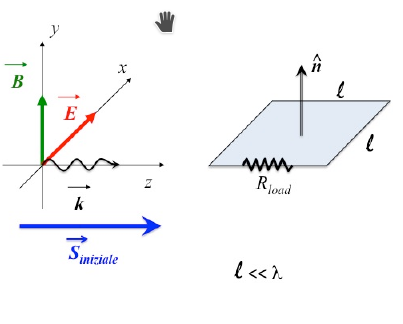
\includegraphics[width=0.5\textwidth]{immagini/spira_onda.png}
	\caption{Spira immersa nel campo di onda e.m.}
	\label{fig:spira1}
\end{figure}
\paragraph{Calcolo della resistenza di irraggiamento.}
I campi ed il vettore di Poynting dell'onda sono:
\[
	\boldsymbol{E} = E_x \hat{i} = E_0 \cos\left( \omega t - kz \right) \hat{i} 
.\] 
\[
	\boldsymbol{B} = B_y \hat{j} = B_0 \cos\left( \omega t - kz \right) \hat{j} 
.\] 
\[
	\boldsymbol{S}_{in} = \frac{E_0^2}{Z_0}\cos\left( \omega t - kz \right) \hat{k} 
.\] 
Sia $I\left( t \right) $ la corrente che scorre nel circuito; possiamo sfruttare le ipotesi di dimensioni piccole (rispetto a $\lambda$) per dire che tale corrente è uniforme in tutta la spira. Trascurando anche autoinduttanza e capacità parassite possiamo affermare che il circuito ha momento di dipolo nullo.\\
Non vale lo stesso per il momento di dipolo magnetico:
\[
	\boldsymbol{p}_m = I\left( t \right) l^2 \hat{j}
.\] 
Adesso aggiungendo le ipotesi di perfetta monocromaticita dell'onda incidente e di nessuna perdita di energia per irraggiamento del circuito si calcola la corrente $I\left( t \right)$ applicando Faraday:   
\[
	\varepsilon\left( t \right) = - \frac{\mbox{d} \Phi\left( \boldsymbol{B} \right) }{\mbox{d} t} = R_{load} I\left( t \right) 
.\]
Mettiamo quindi in mezzo la geometria del circuito:
\[
	I\left( t \right) = \frac{\varepsilon\left( t \right)}{R_{load}} = 
	- \frac{1}{R_{load}} \frac{\mbox{d} \Phi\left( \boldsymbol{B} \right) }{\mbox{d} t} 
	= - \frac{1}{R_{load}} \frac{\mbox{d}}{\mbox{d}t} \left[ \int_{-l/2}^{l/2} B_0 \cos\left( \omega t - kz \right) l dz \right] 
	= \frac{\omega l^2B_0\sin\left( \omega t\right)}{R_{load}} \frac{\sin\left( kl/2 \right)}{kl/2}      
.\] 
Agginungendo l'approssimazione:
\[
	\frac{kl}{2} = \frac{\pi l}{\lambda} \ll 1 \implies I\left( t \right) = \frac{\omega l^2 B_0 \sin\left( \omega t \right) }{R_{load}}  
.\] 
Possiamo allora calcolare la potenza irraggiata:
\[
	P_{el} = \frac{\left| \ddot{\boldsymbol{p_m}} \right| ^2}{6\pi \epsilon_0 c^{5}} = \frac{\ddot{I}^2\left( t \right) l^4}{6\pi \epsilon_0 c^5}
.\] 
Se si effettua un bilancio energetico del circuito:
\[
	\varepsilon I = R_{load}I^2 + P_{el} = R_{load} I^2 + \frac{l^4}{6\pi \epsilon_0 c^5}\ddot{I}^2
.\] 
Nel caso in analisi la f.e.m. è armonica 
\[
	\varepsilon = \varepsilon_0 \sin\left( \omega t \right) \quad 
	\text{ con } \quad  
	\varepsilon_0 = \omega l^2 B_0
\]
Quindi la soluzione stazionaria per la corrente sarà anch'essa armonica: $I = I_0 \sin\left( \omega t \right) $, in conclusione:
\[
	\varepsilon I = R_{load}I^2 + \frac{\omega ^{4}l^{4}}{6\pi \epsilon_0 c^{5}} \implies \varepsilon = \left( R_{load} + R_{irr} \right) I
.\] 
Dove è stata definita la resistenza di irraggiamento (dipendente dalla frequenza):
\[
	R_{irr} = \frac{\omega^4l^4}{6\pi \epsilon_0 c^5}
.\]
Espressa in funzione della lunghezza d'onda:
\[
	R_{irr} = \omega^4 \frac{l^4}{6\pi \epsilon c^5} = \left( \frac{2\pi c}{\lambda} \right) ^4 \frac{l^4\sqrt{\mu_0 \epsilon_0} }{6 \pi \epsilon_0 c^4} = \frac{8}{3}\pi^3 Z_0\left( \frac{l}{\lambda} \right)^4 = 31.1 \text{ k}\Omega \left( \frac{l}{\lambda} \right)^4  
.\] 
\paragraph{Calcolo delle sezioni d'urto.}
Notando che 
\[
	I\left( t \right) = \frac{\varepsilon\left( t \right) }{\left( R_{load} + R_{irr} \right) }
.\] 
Possiamo ottenere la potenza assorbita e la potenza "elastica":
\[
	P_{abs} = R_{load} I^2 = \frac{R_{load}}{\left( R_{load} + R_{irr} \right) ^2}\varepsilon^2
.\] 
\[
P_{el} = R_{irr} I^2 =  \frac{R_{load}}{\left( R_{load} + R_{irr} \right) ^2}\varepsilon^2
.\] 
Quindi la potenza trasferita al carico è massima per $R_{load} = R_{irr}$.\\
Adesso basta mediare il vettore di Poynting per concludere:
\[
\left< \left| \boldsymbol{S}_{in} \right| \right> = \frac{\boldsymbol{E}_0^2}{2Z_0}
.\] 
llora le sezioni d'urto sono:
\[
	\sigma_{abs} = \frac{4\pi^2}{\lambda^2}l^4Z_0 \frac{R_{load}}{\left(R_{load} + R_{irr}\right)^2}
.\] 
\[
	\sigma_{irr} = \frac{4\pi^2}{\lambda^2}l^4Z_0 \frac{R_{irr}}{\left(R_{load} + R_{irr}\right)^2}
.\]
\[
	\sigma_{tot} = \sigma_{irr} + \sigma_{load} = \frac{4\pi^2}{\lambda^2}l^4Z_0 \frac{Z_0}{\left(R_{load} + R_{irr}\right)^2}
.\] 

\subsection[]{ Utilizzando le apposite tabelle che forniscono le masse dei nuclei, determinare il Q-valore o l'energia di soglia dei seguenti processi, valutando l'eventuale ruolo della interazione coulombiana nello stato iniziale:
\begin{enumerate}	
	\item	p + 40Ar $\implies$ p + 39Ar + n 
	\item	p + 14N $\implies$ X + n
	\item	p + 16O $\implies$ X + n
	\item	n + 14N $\implies$ 14C + p
	\item	4He + 14N $\implies$ 17O + p
	\item	2H + 3H $\implies$ 4He + n
	\item	2H + 2H $\implies$ 4He + $\gamma$
	\item	p + 198Hg $\implies$ 197Au + p + p
\end{enumerate}
}
Partiamo con un pò di teoria:
\[
	Q = \sum M_{in} - \sum M_{fin} 
.\] 
Se il Q-valore è positivo allora la reazione avviene in modo spontaneo: l'energia di soglia è nulla.\\
Se il Q-valore è negativo allora l'energia di soglia è maggiore di zero e dipende dalla carica del proiettile.
Se la particella proiettile è neutra allora l'energia di soglia è il modulo del Q-valore, altrimenti è necessario calcolare l'energia necessaria a vincere l'interazione columbiana per arrivare al nucleo (essendo le interazioni sopra scritte tutte forti) nel sistema del laboratorio.\\
Per effettuare il calcolo sfruttiamo la conservazione dell'energia e della quantità di moto non relativistiche in una dimensione, chiariamo la notazione:
\begin{itemize}
	\item $R$: raggio del nucleo colpito 
	\item $m_{prt}$: massa del proiettile.
	\item v$_0$: velocità iniziale del proiettile.
	\item $T$: energia cinetica iniziale del proiettile.
	\item $Z$: protoni del nucleo colpito.
	\item  $M$: massa del nucleo colpito.
	\item $d$: distanza in cui i nuclei si urtano definita dalla somma dei raggi delle due particelle coinvolte:
		 \[
			 d = R + r_{prt} \approx \left( 1.25 A^{1/3} + r_{\text{skin}} + r_{prt} \right) \text{ fm} = \left( 1.25 A^{1/3} + 2 + r_{prt} \right) \text{ fm}  
		.\] 
\end{itemize}
Facendo il conto:
 \[
\begin{cases}
	m_{prt}\text{v}_0 = \left( m_p + M \right)V_{cm}\\
	T \ge \frac{1}{2}\left( m_{prt} + M \right)V_{cm} + \frac{Ze^2}{4\pi \epsilon_0 d} \\
	T = \frac{1}{2}m_{\text{prt}}\text{v}_0^2
\end{cases}
\]
Quindi sviluppando per $T$ si ottinene l'energia cinetica necessaria per la reazione:
\[
	T \ge \left( 1 + \frac{m_{prt}}{M} \right) \frac{Ze^2}{4\pi \epsilon_0 d} = T_{\text{min}} 
.\] 
e per l'energia di soglia dobbiamo soltanto sommare il modulo del Q-valore:
\[
	E_{\text{soglia}} = T_{\text{min}} + \left| Q \right| 
.\] 
In questo modo possiamo risolvere tutte le interazioni elencate.

\paragraph{Interazione 1.}
Bisogna notare che $40 \text{Ar} = \ce{^{40}_{18}\text{Ar}}$ (vedi tabelle con difetti di massa), quindi:
\[
	\ce{p + 40\text{Ar} -> p + 39\text{Ar} + n}
.\] 
\[
	Q = \left( m_p + 40m_u + \Delta_{40, 18} \right) - \left( m_p + 39 m_u + \Delta_{39, 18} + m_n  \right) = m_u + \Delta_{40, 18} - \Delta_{39, 18} - m_n      
.\]
Numericamente:
\[
	Q \approx \left( 931.49 + \left( -35.04 \right) - \left( -33.24 + 939.57 \right)  \right)\text{Mev} \approx -8.3 \text{ MeV} \quad \quad \text{Reazione endotermica}
.\]
Per il calcolo dell'energia di soglia applichiamo subito quando visto sopra:
\[
	E_{\text{soglia}} = \left( 1 + \frac{m_p}{M_{40\text{Ar}}} \right) \frac{Ze^2}{4 \pi \epsilon_0 d} + \left| Q \right| \quad \quad 
	\text{con } M_{40Ar} = 40m_u + \Delta_{40,18}
.\]
si calcola la distanza minima d (il raggio del protone è circa 1.25 fm): 
\[
	d \approx \left( 1.25 \cdot \left( 40 \right)^{ 1/3 } + 2 + r_{protone} \right)\text{fm} \approx 6.25 \text{ fm} 
.\] 
Quindi l'energia di soglia (calcolo numerico approssimato a mente\ldots):
\[
	E_{\text{soglia}} \approx 4 \text{ MeV} + 8 \text{ MeV} \approx 12 \text{ MeV}   
.\] 
Analogamente per le altre reazioni.

\subsection[]{  Dimostrare la relazione fra la definizione della sezione d’urto elastica nel caso di fotoni incidenti su un unico bersaglio e la definizione di sezione d'urto elastica per un’onda e.m. monocromatica su un unico bersaglio.}
Nel caso di onda monocromatica su un bersaglio si ha:
\[
	\sigma_{\text{el}} = \frac{\left< P_{el}\right>}{\left<\left| \boldsymbol{S}_{in} \right|  \right>}
.\]
Mentre per un fascio di fotoni incidenti:
\[
	\sigma_{\text{el}} = \frac{\frac{\mbox{d} N_{el}}{\mbox{d} t}}{\left| \boldsymbol{j}_{\gamma}\right|}
.\] 
L'equivalenza delle due deriva dal fatto che se si moltiplica e si divide la seconda per $ \hbar \omega$:
\[
	\sigma_{\text{el}} = \frac{\frac{\mbox{d} N_{el}}{\mbox{d} t}}{\left| \boldsymbol{j}_{\gamma}\right|} = \frac{\frac{\mbox{d} N_{el}}{\mbox{d} t}\hbar \omega }{\left| \boldsymbol{j}_{\gamma}\right|\hbar \omega} = \frac{\left< P_{el}\right>}{\left<\left| \boldsymbol{S}_{in} \right|  \right>}
.\] 	

\subsection[]{  Quale calcolo si deve effettuare per determinare il numero di eventi per unità di tempo e di volume che si producono negli urti fra particelle di due specie diverse e differenti concentrazioni le cui velocità relative sono distribuite con un funzione $f(V_{rel})$, normalizzata all'unità, e la cui sezione d'urto è $\sigma(V_{rel})$?}
Date due specie con densità volumica $n_a$ e  $n_b$ che si scontrano e con densità di prodotti $n_f$, se la $ f\left( V_{\text{rel}} \right) $ è normalizzata allora si ha:
\[
	\frac{\mbox{d} n_{\text{f}}}{\mbox{d} t } = n_a n_b \int_0^{\infty} f\left( v_{rel} \right) \sigma_{\text{f}}\left( v_{rel} \right) v_{rel} dv_{rel}
.\] 
Tipicamente la $f\left( V_{rel} \right)$ è gaussiana. 

\subsection[]{ Calcolare l'attenuazione di un fascio di particelle incidenti su un materiale omogeneo e composto da atomi di una sola specie in funzione della profondità [dati: sezione d'urto del processo su ogni atomo del bersaglio, densità di massa del mezzo, numero atomico del mezzo].}
\label{sec:2.b.5}
\paragraph{Lamina sottile}
Data una lastra di materiale omogeneo definiamo alcune (tante, forse troppe) quantità utili: spessore $\Delta x$, densità $\rho$, area $\Delta S$, volume di lastra considerato $V$ , sezione d'urto su ogni atomo bersaglio (totale) $ \sigma_{\text{tot}}$, $n_b$ la concentrazione di besagli nel materiale e $n_a$ la concentrazione di particelle incidenti. Possiamo riscrivere queste in funzione delle quantità date dal testo e sfruttare qualche utile relazione.\\ 
Partiamo da $n_b$: definendo $M_{\text{tot}}$ la massa totale di lastra nel volume, $M_A$ la massa di una mole della sostanza del materiale in grammi, $N_a$ il numero di avogadro si ha:
\[
	V \cdot n_b = N_{\text{tot}} = \frac{M_{\text{tot}}}{M_A} N_a \implies n_b =\frac{N_{\text{tot}}}{V} = \frac{\rho}{M_A} N_a
.\]
La probabilità di interazione nel volume considerato è definita da:
\[
	P_{\text{int}} = n_b \cdot \sigma_{\text{tot}} \Delta x  = \frac{\rho N_a }{M_A} \sigma_{\text{tot}}\Delta x
.\] 
A questo punto si vede come è definita la profondità di penetrazione (essendo la $P_{\text{int}}$ adimensionale):
\[
	\mathcal{L} = \frac{M_A}{\rho N_a\sigma_{\text{tot}}}
.\] 
quindi l'attenuazione è data dalla frazione di particelle che riescono a passare, quantità che si può ricavare come il complementare della probabilità di interagire: la probabilità di passare.
\[
	A = 1 - \frac{\Delta x}{\mathcal{L}} \quad \quad 
	\text{Nel caso di lamina sottile}
.\] 
Quanto visto fin'ora funziona finche la lamina si può considerare sottile: $\Delta x < \mathcal{L}$, se questa approssimazione viene meno è necessario rivedere alcuni conti.
\paragraph{Materiale generico} Possiamo pensare ad un materiale generico come la sovrapposizione di tante lamine sottili di diversa superficie. Si può quindi vedere la probabilità di interazione come una funzione della posizione $P_{\text{int}}\left( x \right)$, quindi anche la stessa attenuazione sarà funzione della posizione $A\left( x \right) $. Calcoliamo l'attenuazione alla posizione $x + \Delta x$, dobbiamo utilizzare le regole delle probabilità combinate:
\[
	A\left( x + \Delta x \right) = A\left( x \right) A\left( \Delta x \right) = A\left( x \right) \left( 1- P_{\text{int}}\left( \Delta x \right)  \right) = A\left( x \right) \left( 1 - \frac{\Delta x }{\mathcal{L}} \right)  
.\]
Applicando il rapporto incrementale risulta quindi evidente che il risultato sarà esponenziale ( cosa che goffamente sapevamo già dal momento che si applicano le proprietà della probabilità di eventi ripetuti).
\[
	\frac{A_{\text{int}}\left( x + \Delta x \right) - A_{\text{int}}\left( x \right)}{\Delta x} = -\frac{A\left( x \right) }{\mathcal{L}} 
.\]
Facendo tentere $\Delta x$ a zero:
\[
	\dot{A} = -\frac{A}{\mathcal{L}} \implies A\left( x \right) = e^{-x/\mathcal{L}} \quad \quad 
	\text{Materiale generico}
.\] 

\subsection[]{  Calcolare l'attenuazione di un fascio di particelle incidenti su un materiale omogeneo e composto da atomi di diverse specie in funzione della profondità [dati: sezione d'urto del processo su ogni atomo del bersaglio, densità di massa del mezzo, numeri atomici, composizione chimica del mezzo]}
\paragraph{Lamina sottile}
Essendo nota la composizione chimica del mezzo è noto anche la percentuale di atomi che compongono il materiale:
\[
	\text{Composizione del mezzo: } \ X^{\left( 1 \right) }_{a_1}\ldots X^{(N)}_{a_N}
.\]
Con $X^{i}$ specie atomica, $a_j$ pedice che indica la composizione chimica nella formula del composto (per non appesantire si trascurano le formule con simboli ripetuti tipo $CH_3COOH$).
Si può quindi ragionare come se avessimo N copie del nostro materiale ognuno interamente composto da una singola specie preservando le densità $\rho_i$ che sono presenti nel materiale originale, successivamente si applica il principio di sovrapposizione sommando tutte le attenuazioni e normalizzando sulle N specie:
\[
	A_i = 1 - \frac{\Delta x}{\mathcal{L}_i} \implies A_{\text{tot}} = \frac{\sum_{n=1}^{N} A_n}{N} = 1 - \sum_{n=1}^{N} \frac{\Delta x}{N \mathcal{L}_n}
.\] 
con la penetrazione definita a partire dalla densità e dalla massa molare delle singole specie:
\[
	\mathcal{L}_i = \frac{M_{A}^{\left( i \right) }}{\rho_i N_a \sigma_{\text{tot}}}
.\]
\paragraph{Materiale generico}
Con passaggi del tutto analoghi alla domanda precedente si arriva alla conlcusione:
\[
	A_{\text{tot}} =\frac{\sum_{n=1}^{N} e^{-x/\mathcal{L}_n}}{N} 
.\] 
\subsection[]{  Effettuare una stima numerica della sezione d'urto totale forte per i seguenti urti: 
\begin{enumerate}
	\item	p + 40Ar
	\item	n + 14N
	\item	4He + 14N
	\item	2H + 3H
\end{enumerate}
}
Se si considera solo la sezione d'urto forte non c'è bisogno di preoccuparsi di interazioni elettrodeboli: si suppone che l'energia sia sufficiente da poter trascurare questo tipo di interazioni. Il calcolo si riduce alla stima della superficie di possibile impatto tra i due oggetti assunti come sferici:
\[
	\sigma_{\text{strong}} \approx \pi\left( R_1 + R_2 \right)^{2} 
.\] 
Con $R_1$ e  $R_2$ raggi delle particelle interagenti. Per tutti gli atomi in gioco ho scelto di considerare sempre $r_\text{skin}$.
\paragraph{Interazione 1.}
\[
	\sigma_1 \approx \pi\left( r_p + R_{40\text{Ar}} \right)^{2}  \approx \pi (1.25 \cdot (40)^{1/3} + 2 + 1.25 )^{2} \text{ fm}^{2} \approx \pi \cdot (6.25)^{2} \text{ fm}^{2}
\]
Quindi 
\[
	\sigma_1 \approx \pi \cdot 39 \text{ fm}^{2} \approx 120 \text{ fm}^{2} = 1.2 \text{b}
\]
\paragraph{Interazione 2.} 
$\sigma_2 \approx 1.23 \text{b}$

\paragraph{Interazione 3.}
$\sigma_3 \approx 2.54 \text{b} $

\paragraph{Interazione 4.}
$\sigma_4 \approx 1.7 \text{b}$

\subsection[]{  Calcolare l’energia che dovrebbe avere un protone che incide su un protone fermo per ottenere una energia nel centro di massa pari a quella di LHC (14TeV).}
Sia $E$ l'energia del protone nel laboratorio, si ha:
\[
	E^2_{\text{cm}} = \left( E_{lab} \right)^{2} -  \boldsymbol{P}_{\text{lab}}^{2} = \left( E + m_p \right)^{2} - \left(E^2 - m_p^2\right) = 2m_p^2 + 2m_pE 
.\]
Quindi l'energia necessaria è circa $E = 10^{6} $ TeV

\subsection[]{ Calcolare l'energia di degli elettroni/positroni per innescare la reazione:
\[
	e^{+} \ + \ e^{-} \implies p \ + \ \overline{p}
\] 
in cui i due leptoni collidono con 3-impulsi opposti e di modulo diverso.}

Se $E_1$ e $E_2$ sono le energie dei due leptoni si ha 
\[
	\left( E_1 + E_2 \right) ^2 - \left( \sqrt{E_1^2 - m_e^2} - \sqrt{E_2^2 - m_{e}^2}  \right) \ge 4 m_p^2
.\]
L'energia di soglia si ottinene studiando la funzione nelle due variabili sopra, da lì si evince che il minimo si ha per $E_1 = E_2$, quindi:
\[
	E_{\text{min}} = m_p
.\] 

\subsection[]{ Calcolare l’energia di soglia nel laboratorio per le seguenti reazioni (la seconda particella è inizialmente ferma):
\begin{enumerate}
	\item	$\gamma \ + \ {}^{16} O \implies e^{+} \ + \ e^{-} \ + \ {}^{16}O $
	\item	$\gamma \ + \ e^{-} \implies e^{-} \ + \ e^{+} \ + \ e^{-}$
	\item	$p \ + \ p \implies p \ + \ p \ + \ p \ + \ \overline{p}$
	\item	$p \ + \ {}^{16}O \implies p \ + \ p \ + \ \overline{p} \ + \ {}^{16}O$
	\item	$e^{+} \ + \ e^{-} \implies p \ + \ \overline{p}$
	\item	$e^{-} \ + \ p \implies n \ + \ \nu_e$
	\item	$\overline{\nu_e} \ + \ p  \implies n \ + \ e^{+}$
\end{enumerate}
}

Per tali calcoli è necessaria una generalizzazione della risposta al quesito precedente, è infatti richiesto che:
\[
	\left( \sum_i P_{i,\text{in}} \right)^2 \ge \left(\sum_{i} m_{i, \text{fin}} \right)^2  
.\] 
Adesso si può sfruttare il fatto che i reagenti sono soltanto due e che il secondo è sempre a riposo (generalizzazione della domanda 2.b.8):
\[
	E_1 \ge \frac{1}{2m_2}\left[ \left( \sum_{i} m_{i, \text{fin}} \right)^2 - \left( m_1^2 + m_2^2 \right)  \right] 
.\]
E adesso si tratta solo di infilare dentro i numeri.

\subsection[]{ Calcolare la probabilità che un neutrino interagisca nell’attraversare la Terra lungo un diametro.\\
Nota: sia assuma che l’energia del neutrino sia tale che la sezione d’urto totale su un singolo nucleone sia 1 fb. } 
Si assume per il calcolo $\rho_{\text{T}} \approx 5.5 \text{g}/\text{cm}^3$.\\
Possiamo ipotizzare una bassa probabilità di interazione per il neutrino, è quindi possibile assumere la terra come una lamina sottile (con immenso piacere dei terrapiattisti) e calcolare la probabilità cercata come:
\[
P_{\text{int}} = n \sigma d \approx 4.2 \cdot 10^{-5} 
.\] 
Con $d \approx 12.76 \cdot 10^{3} \text{ km}$ raggio terrestre e $n \approx \rho_{\text{T}}\cdot N_A\cdot A / M_{\text{Si}} = \rho\cdot N_{\text{A}} / 1 \text{[g]} \approx 5.5\cdot 6 \cdot 10^{23} \text{cm}^{-3}$ densità media della terra (composta principalmente da Silicio).

\subsection[]{ Dimostrare che un elettrone (non relativistico) soggetto ad una forza elastica di richiamo, ad una forza di attrito viscoso ed alla forza di reazione radiativa, nel campo di un’onda e.m. piana polarizzata linearmente oscilla con la legge:
\[
	\boldsymbol{x} = \frac{e \boldsymbol{E_0}}{m_{e}} \frac{1}{\omega_0^2-\omega^2-i\omega\Gamma_{tot}} e^{-i \omega t} \quad \quad 
	\text{ con }  \quad \quad
	\Gamma_{tot} = \Gamma' + \Gamma \frac{\omega^2}{\omega_{0}^2}
\] 
} \label{subsec: 2.b.12}
Facendo riferimento ai risultati delle Domande \hyperref[subsec: 2.a.15]{2.a.15}, \hyperref[subsec: 2.a.16]{2.a.16}  si prosegue con il calcolo.
L'equazione di moto dell'elettrone in questo caso è (considerando anche la $F_{\text{rad}}$):
\[
m_e \ddot{\boldsymbol{x}} = q \boldsymbol{E_0}e^{-i \omega t} - m_e \tau \dddot{\boldsymbol{x}} - m_e \Gamma' \dot{\boldsymbol{x}}
.\] 
Spostando l'incognita vettoriale a destra si ha:
\[
-\tau \dddot{\boldsymbol{x}} + \ddot{\boldsymbol{x}} + \Gamma' \dot{\boldsymbol{x}} + \omega _0^2 \boldsymbol{x} = \frac{q \boldsymbol{E_0}}{m_e} e^{-i \omega t}
.\] 
Cercando la soluzione stazionaria $\boldsymbol{x} = \boldsymbol{x}_0 e^{-i \omega t}$ si ha:
\[
	-\tau \left( -i \omega \right)^3 \boldsymbol{x}_0e^{-i \omega t} + \left( - i \omega \right) \Gamma'\boldsymbol{x}_0 e^{-i \omega t} + \omega _0^2 \boldsymbol{x}_0 e^{-i \omega t} = \frac{q \boldsymbol{E}_0}{m_e} e^{-i \omega t}
.\] 
Quindi:
\[
\boldsymbol{x}_0 = \frac{q \boldsymbol{E}_0/m_e}{ \omega _0^2 - \omega ^2 -i \omega \Gamma' - i \tau \omega ^2 }
.\]
È quindi utile definire $\Gamma_{\text{tot}} = \Gamma' + \tau \omega ^2 = \Gamma' + \Gamma \frac{\omega ^2}{\omega _0^2}$ per giungere alla conclusione:
\[
\boldsymbol{x} = \frac{q \boldsymbol{E}_0}{m_e} \frac{e^{-i \omega t}}{\omega _0^2 - \omega ^2 - i \omega \Gamma_{\text{tot}}} 
.\] 

\subsection[]{Dimostrare che la sezione d’urto differenziale elastica per un’onda e.m. piana e monocromatica su un elettrone legato elasticamente vale 
\[
	\frac{\mbox{d} \sigma_{el}}{\mbox{d} \Omega} = r_e^2 L\left( \omega \right) \sin^2\left( \alpha  \right)    
\]
con $\alpha$ angolo fra la direzione di osservazione e direzione di polarizzazione (lineare) dell'onda.} \label{subsec: 2.b.13}
La risposta al quesito è stata prematuramente scritta alla Domanda \hyperref[subsec: 2.a.16]{2.a.16} facendo uso del risultato ottenuto nella Domanda \ref{subsec: 2.b.12}.
Si riaccenna solo al fatto che è stata definita $L\left( \omega  \right)$ come:
\[ 
	L \left( \omega \right) = \frac{\omega^4}{\left( \omega_{0}^2 - \omega^2 \right)^2 + \omega^2 \Gamma_{tot} } \quad \quad 
.\] 
Vediamo di dimostrare quanto scritto, sopra abbiamo ottenuto:
\[
\boldsymbol{x} = \frac{q \boldsymbol{E}_0}{m_e} \frac{e^{-i \omega t}}{\omega _0^2 - \omega ^2 - i \omega \Gamma_{\text{tot}}} 
.\] 
Calcoliamo il vettore di Poynting (mediato nel tempo) associato alla potenza irraggiata dall'elettrone:
Esplicitando l'espressione del .. in funzione della variabile $\alpha$ del problema si ha:
\[
	\boldsymbol{E_{\text{dip}}} =k_0 \frac{\left( e\ddot{\boldsymbol{x}} \wedge \hat{r}\right) \wedge \hat{r}}{\left| \boldsymbol{r} \right| c^2} 
.\] 
\[
	\left<\boldsymbol{S}_{\text{el}} \right> = \left< \boldsymbol{E} \wedge H\right> = \left<\frac{\left| \boldsymbol{E}_{\text{dip}} \right|^2}{c \mu_0}  \right> = 
	k_0^2\frac{\left| e \ddot{\boldsymbol{x}}  \right|^2 \sin^2\left( \alpha  \right) }{c^4 r^2 \mu_0 } =
	\frac{1}{32 \pi^2 \epsilon_0} \frac{ \left| e \ddot{\boldsymbol{x}}_0 \right|^2 \sin^2\left( \alpha \right) }{c^3 r^2} \hat{r}
.\] 
Che in CGS risulta più elegante:
\[
\left<\boldsymbol{S}_{\text{el}} \right> = \frac{1}{8 \pi} \frac{ \left| e \ddot{\boldsymbol{x}}_0 \right|^2 \sin^2\left( \alpha \right) }{c^3 r^2} \hat{r} 
.\] 
Dividendo questo vettore per il vettore di poynting iniziale (da qui in poi CGS per semplicità) si ottiene l'espressione cercata:
\begin{align*}
\frac{\mbox{d} \sigma_{\text{el}}}{\mbox{d} \Omega} = \frac{\left< \boldsymbol{S}_{\text{el}} \right> \cdot r^2 \hat{r}}{\frac{c}{8 \pi}\left| E_0 \right|^2 } = 
\frac{ \omega^{4} e^{4}}{c^{4}m_e^2} \frac{\sin^2\left( \alpha  \right) }{\left( \omega _0^2 - \omega ^2 \right)^2 + \omega ^2 \Gamma_{\text{tot}}^2} =
r_e^2 \frac{\omega ^{4}\sin^2\left( \alpha \right)}{\left( \omega _0^2 - \omega ^2 \right)^2 + \omega ^2 \Gamma_{\text{tot}}^2}
.\end{align*}
Dove è necessario riconoscere il raggio classico in CGS:
\[
	r_e^{\left( \text{CGS} \right) } = \frac{e^2}{c^2m_e}
.\] 
Va da se che in MKSA:
\[
	\frac{\mbox{d} \sigma_{\text{el}}}{\mbox{d} \Omega} = \left( \frac{k_0 e^2}{m_e c^2} \right) ^2 \frac{\omega ^{4}\sin^2\left( \alpha \right)}{\left( \omega _0^2 - \omega ^2 \right)^2 + \omega ^2 \Gamma_{\text{tot}}^2}
.\] 

%2.b.14
\subsection[]{Dimostrare che la sezione d’urto Thomson vale $\sigma_{Th} = \frac{8}{3}\pi r_{e}^2  = 0.66 \text{ barn}$.}
Si può arrivare allo Scattering Thompson riscrivendo l'equazione di moto dell'elettrone e trascurando la pressione di radiazione di cui si è invece fatto uso nelle precedenti domande:
\[
m_e \ddot{\boldsymbol{x}}= e \boldsymbol{E}_0 e^{-i \omega t}
.\] 
La potenza irraggiata di dipolo sarà quindi:
\[
P_{\text{irr}} = k_0 \frac{e^2 \left| \ddot{\boldsymbol{x}} \right|^2}{3c^3} 
.\]
Sviluppando i conti e ricordando la definizione di sezione d'urto si arriva banalmente a:
\[
\sigma_{\text{Th}}=\frac{8}{3}\pi r_e^2
.\] 
Ricordando ancora che il \hyperref[eq: raggio classico]{Raggio classico dell'elettrone} è: $r_e = k_0 \frac{e^2}{m_e c^2} \approx 2.82$ fm.

%2.b.15
\subsection[]{Dimostrare che la sezione d’urto elastica per un’onda e.m. piana e monocromatica su un elettrone legato elasticamente vale:
\[
	\sigma_{el} = \sigma_{Th} L\left( \omega \right) 
\] 
}
È in pratica richiesto di trovare la Funzione di Brieght-Wiegner. Visto che abbiamo la sezione differenziale tuttavia è sufficiente integrarla su tutti gli angoli. Ci si riduce allora al calcolo dell'integrale:
\[
	\int \sin^2\left( \alpha  \right) d \Omega = \int \frac{1 + \cos^2\left( \alpha \right) }{2} d\Omega = 2\pi + \frac{1}{2} 2 \pi \int_0^{2\pi} \cos^2\left( \alpha  \right) \sin\left( \alpha  \right) d \alpha = \frac{8}{3}\pi  
.\] 
Tutto il resto esce indisturbato dall'integrale sull'angolo solido, da cui la tesi.

%2.b.16
\subsection[]{Dimostrare che la sezione d’urto totale per un’onda e.m. piana e monocromatica su un elettrone legato elasticamente vale:
\[
		\sigma_{\text{tot}} = 4 \pi r_{e} c L\left( \omega \right)
\] 
}
Abbiamo gia risolto l'equazione del moto:
\[
\boldsymbol{x}= \frac{e \boldsymbol{E}_0}{m} \frac{e^{- i \omega t}}{\omega _0^2 - \omega ^2 - i \omega \Gamma_{\text{tot}}}
.\] 
Si tratta quindi solo di ricordare che la potenza totale dissipata può essere espressa come:
\[
	P_{\text{tot}} = \left<\boldsymbol{v} \cdot \boldsymbol{F} \right> = \left<\dot{\boldsymbol{x}}\cdot q \boldsymbol{E} \right> = \left< e \dot{\boldsymbol{x}} \cdot \boldsymbol{E} \right> = \frac{1}{2} q \mathcal{R}e \left\{ \dot{\boldsymbol{x}} \cdot \boldsymbol{E}^* \right\} 
.\]
Quindi:
\[
	P_{\text{tot}} = \frac{q^2 \omega ^2 \left| \boldsymbol{E}_0 \right|^2 \Gamma_{\text{tot}}}{2m\left( \left(\omega _0^2 - \omega ^2 \right) ^2 + \omega ^2 \Gamma_{\text{tot}}^2  \right) }
.\] 
Resta adesso da dividere per il vettore di Poynting incidente:
\[
\sigma_{\text{tot}} = \frac{P_{\text{tot}}}{\left<\left| \boldsymbol{S}_{\text{in}} \right|\right>} = 4 \pi r_{e} c L\left( \omega \right) 
.\] 
Per completezza si scrive anche:
\[
\sigma_{\text{abs}} = \sigma_{\text{tot}} - \sigma_{\text{el}} = 4 \pi r_{e} \omega^2 L\left( \omega \right) \left[ e \Gamma_{\text{tot}} - \frac{2}{3}r_e \omega^2 \right]
.\] 
\begin{figure}[H]
	\centering
	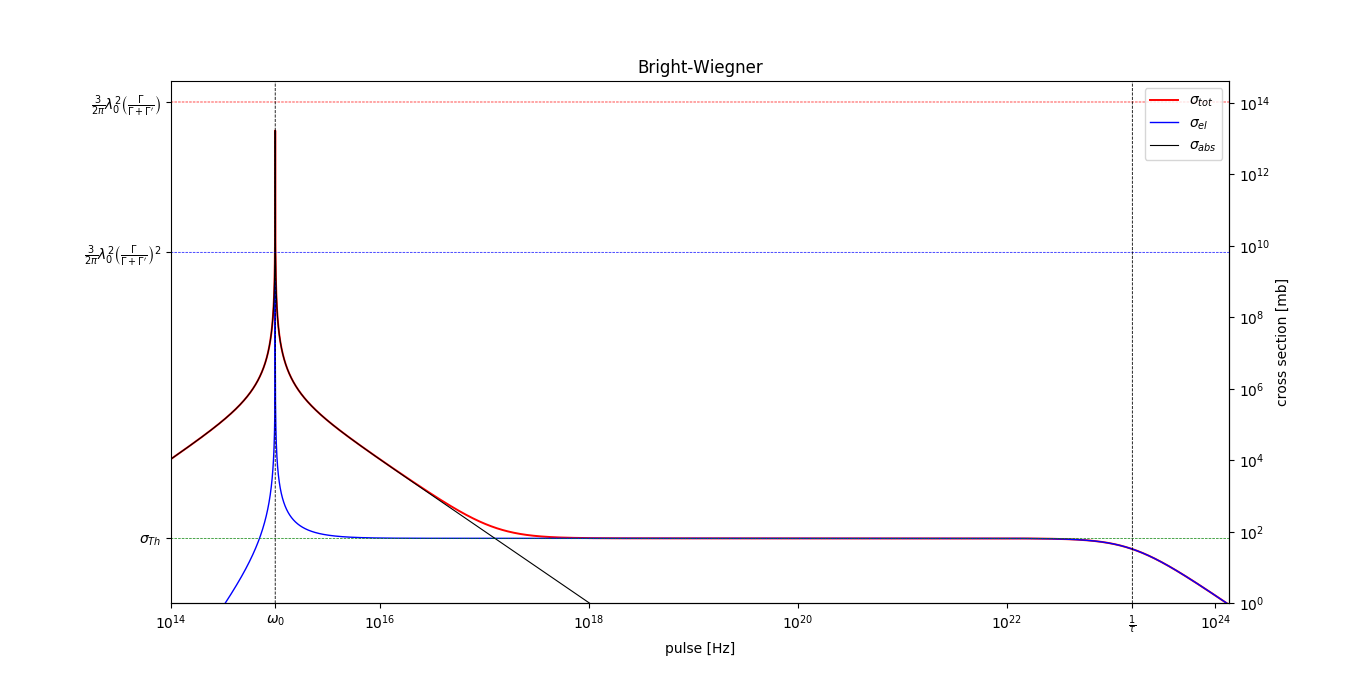
\includegraphics[width=1.1\textwidth]{immagini/b-w.png}
	\caption{Andamento delle sezioni d'urto della Bright-Wiegner}
	\label{fig:Andamento Bright-Wiegner}
\end{figure}
Nella figura si mostra come vanno le sezioni d'urto, è necessario notare che, per un rendering più fedele, sarebbero serviti più punti plottati (la funzione non ha raggiunto il massimo atteso). Per pigrizia è stato testato che arrivasse al massimo ma non è stata riportata l'immagine; insomma fidarsi o provare per credere.

%2.b.17
\subsection[]{Dimostrare che la sezione d’urto elastica per un’onda e.m. piana e monocromatica su un elettrone legato elasticamente in prossimità di una risonanza stretta (specificare il criterio) si può approssimare con una curva lorentziana
\[
	\sigma_{el} = \sigma_{Th} \frac{\omega_{0}^2 / 4}{ \left( \omega_0 - \omega \right)^2 + \frac{ \left( \Gamma' + \Gamma  \right)^2 }{4} }
\] 
}
La B-W si approssima con una lorenziana in un intorno (dell'ordine della larghezza $\Gamma + \Gamma'$) di $\omega_0$: $\omega \approx \omega_0$.\\
La risonanza è stretta se la larghezza a metà altezza è molto inferiore alla frequenza di risonanza: $\Gamma + \Gamma' \ll \omega_0$.
Passiamo alle approssimazioni allora:
\begin{align*}
	\sigma_{\text{el}} = \sigma_{\text{Th}}\frac{\omega ^{4}}{\left( \omega _0 - \omega\right)^2 \left( \omega_0 + \omega \right)^2 + \omega^2\left( \Gamma + \Gamma' \frac{\omega^2}{\omega_0^2} \right)^2} \approx \\
	\approx \sigma_{\text{Th}} \frac{\omega _0^4}{4 \omega _0^2 \left( \omega _0 - \omega  \right)^2 + \left( \Gamma + \Gamma' \right)^2 \omega _0^2  } \approx \\
	\approx \sigma_{\text{Th}}\frac{\omega_0^2/4}{\left( \omega - \omega_0 \right)^2 + \left(\frac{\Gamma + \Gamma'}{2}\right)^2 }
.\end{align*}

% 2.b.18
\subsection[]{Dimostrare che per un’onda e.m. piana e monocromatica su un elettrone legato elasticamente le sezioni d'urto al picco valgono:
\[
	\sigma_{el} = \frac{3 \lambda_{0}^2}{2 \pi} \left( \frac{\Gamma}{\Gamma + \Gamma'} \right)^2 \quad \quad \quad \quad \quad \quad \text{ }
\]
\[
	\sigma_{TOT} = \frac{3 \lambda_{0}^2}{2 \pi} \frac{\Gamma}{\Gamma + \Gamma'} \quad \quad \text{Con $\lambda_{0} = \frac{2 \pi c}{\omega_{0}}$}
\]
\[
	\sigma_{inel} = \frac{3 \lambda_{0}^2}{2 \pi} \frac{\Gamma \Gamma'}{\left( \Gamma + \Gamma' \right)^2 } \quad \quad \quad \quad \quad \quad \text{ } 
\]
}
Accettanto il fatto che tutte le tre sezioni d'urto hanno un massimo per $\omega = \omega_0$ basta prendere le sezioni d'urto e sbatterci dentro $\omega = \omega_0$.

%2.b.19
\subsection[]{Dimostrare che un elettrone (moto non relativistico) soggetto ad una forza elastica di richiamo, ad una forza di attrito viscoso ed alla forza di reazione radiativa, se viene lasciato libero di oscillare da una posizione iniziale perde energia con una 1 legge esponenziale in cui la costante tempo vale $\frac{1}{\Gamma' + \Gamma}$. Come si chiama questa costante tempo? Quale sarebbe la costante tempo con cui, invece, si smorza l'ampiezza delle oscillazioni?}
Riprendiamo l'equazione di moto dell'elettrone, tuttavia adesso togliamo la forzante dovuta all'onda incidente.
\[
	- \tau \dddot{\boldsymbol{x}} + \ddot{\boldsymbol{x}} + \Gamma' \dot{\boldsymbol{x}} + \omega_0^2 \boldsymbol{x} = 0 
.\]  
Adesso è necessario ricordare le relazioni tra i vari parametri in gioco:
\[
	\Gamma' \ll \omega_0 \ll \frac{1}{\tau}, \quad \quad \quad  
	\Gamma \ll \omega_0
.\] 
La prima è una questione puramente di grandezze fisicamente tipiche, la seconda deriva dalla prima $\left( \omega_0 \tau \ll 1 \right) $ e dal fatto che $\Gamma = \tau \omega_0^2 \ll 1 \cdot \omega_0$.\\
È quindi ragionevole cercare una soluzione oscillante e smorzante con smorzamento debole rispetto alla pulsazione:
\[
	\boldsymbol{x} = \boldsymbol{x}_0 e^{-i\left( \omega_0 - i \gamma/2 \right)t } = \boldsymbol{x}_0 e^{-i \omega_0t} e^{-\gamma t /2}, \quad \quad \quad 
	\gamma \ll \omega_0
.\]
Adesso la festa è nel sostituire questa soluzione nella equazione buttando via i termini trascurabili:
\[
	- \tau \left( -i\left( \omega_0 - i \gamma /2 \right)  \right)^3 + \left( -i\left( \omega_0 - i \gamma /2 \right) \right)^2 - \left( -i\left( \omega_0 - i \gamma /2 \right) \right) \Gamma' - \omega_0^2 = 0 
.\]
Sostituendo $\tau = \Gamma / \omega_0^2$:
\[
	-i \frac{\Gamma}{\omega_0^2}\left( \omega_0^3 - \frac{3}{2} i \gamma \omega_0^2 + \ldots \right) - \left( \omega_0^2 - i \gamma \omega_0 + \ldots \right) + 
	\left( -i \Gamma' \omega_0 - \frac{1}{2} \gamma \Gamma'  \right) + \omega_0^2 \approx 0 
.\] 
Sempre sulla base delle approssimazioni sopra è possibile notare che i termini reali sono trascurabili (raggruppare alcuni $\Gamma$ o $\Gamma'$ nei punti giusti per vederlo), ci si riduce alla forma:
\[
	-i \Gamma \omega_0 - \frac{3}{2} \Gamma \gamma - i \Gamma' \omega_0 + i \gamma \omega_0 - \frac{1}{2} \gamma \Gamma' \approx 0 \implies 
	- \Gamma \omega_0 - \Gamma' \omega_0 + \gamma \omega_0 \approx 0 
.\] 
Che ci porta alla conclusione:
\[
\gamma \approx \Gamma + \Gamma 
.\]
Quindi l'ampiezza delle oscilazioni è smorzata con una costante tempo data da:
\[
	\boldsymbol{x} = \ldots \cdot e^{- t /\tau_{\text{osc}}} \quad \quad \text{con} \quad \quad
\tau_{osc} = \frac{2}{\gamma} = \frac{2}{\Gamma + \Gamma'}
.\]
Se consideriamo invece l'andamento della energia è necessario tener conto del fatto che essa è quadratica nella velocità (cinetica) e nella posizione (potenziale): 
\[
E = E_0 e^{- \gamma t} \quad \implies \quad \tau_{\text{energia}} = \frac{1}{\gamma} = \frac{1}{\Gamma + \Gamma'}
.\]
In tutto questo macello il risultato importante è uno: la larghezza totale di uno stato risonante è il reciproco della sua vita media, risonanza stretta = particella longeva e viceversa.

% 2.b.20
\subsection[]{Calcolare la relazione tra parametro d'impatto (b) e angolo di scattering ($\theta$) nel caso di scattering di Rutherford (Coulombiano) e di scattering su sfera rigida.} 
\label{sec:2.b.20}
Prima di iniziare con questi argomenti è bene dare una rilucidatà ad alcune grandezze tipiche in esame: le dimensioni atomiche.
\begin{figure}[H]
	\centering
	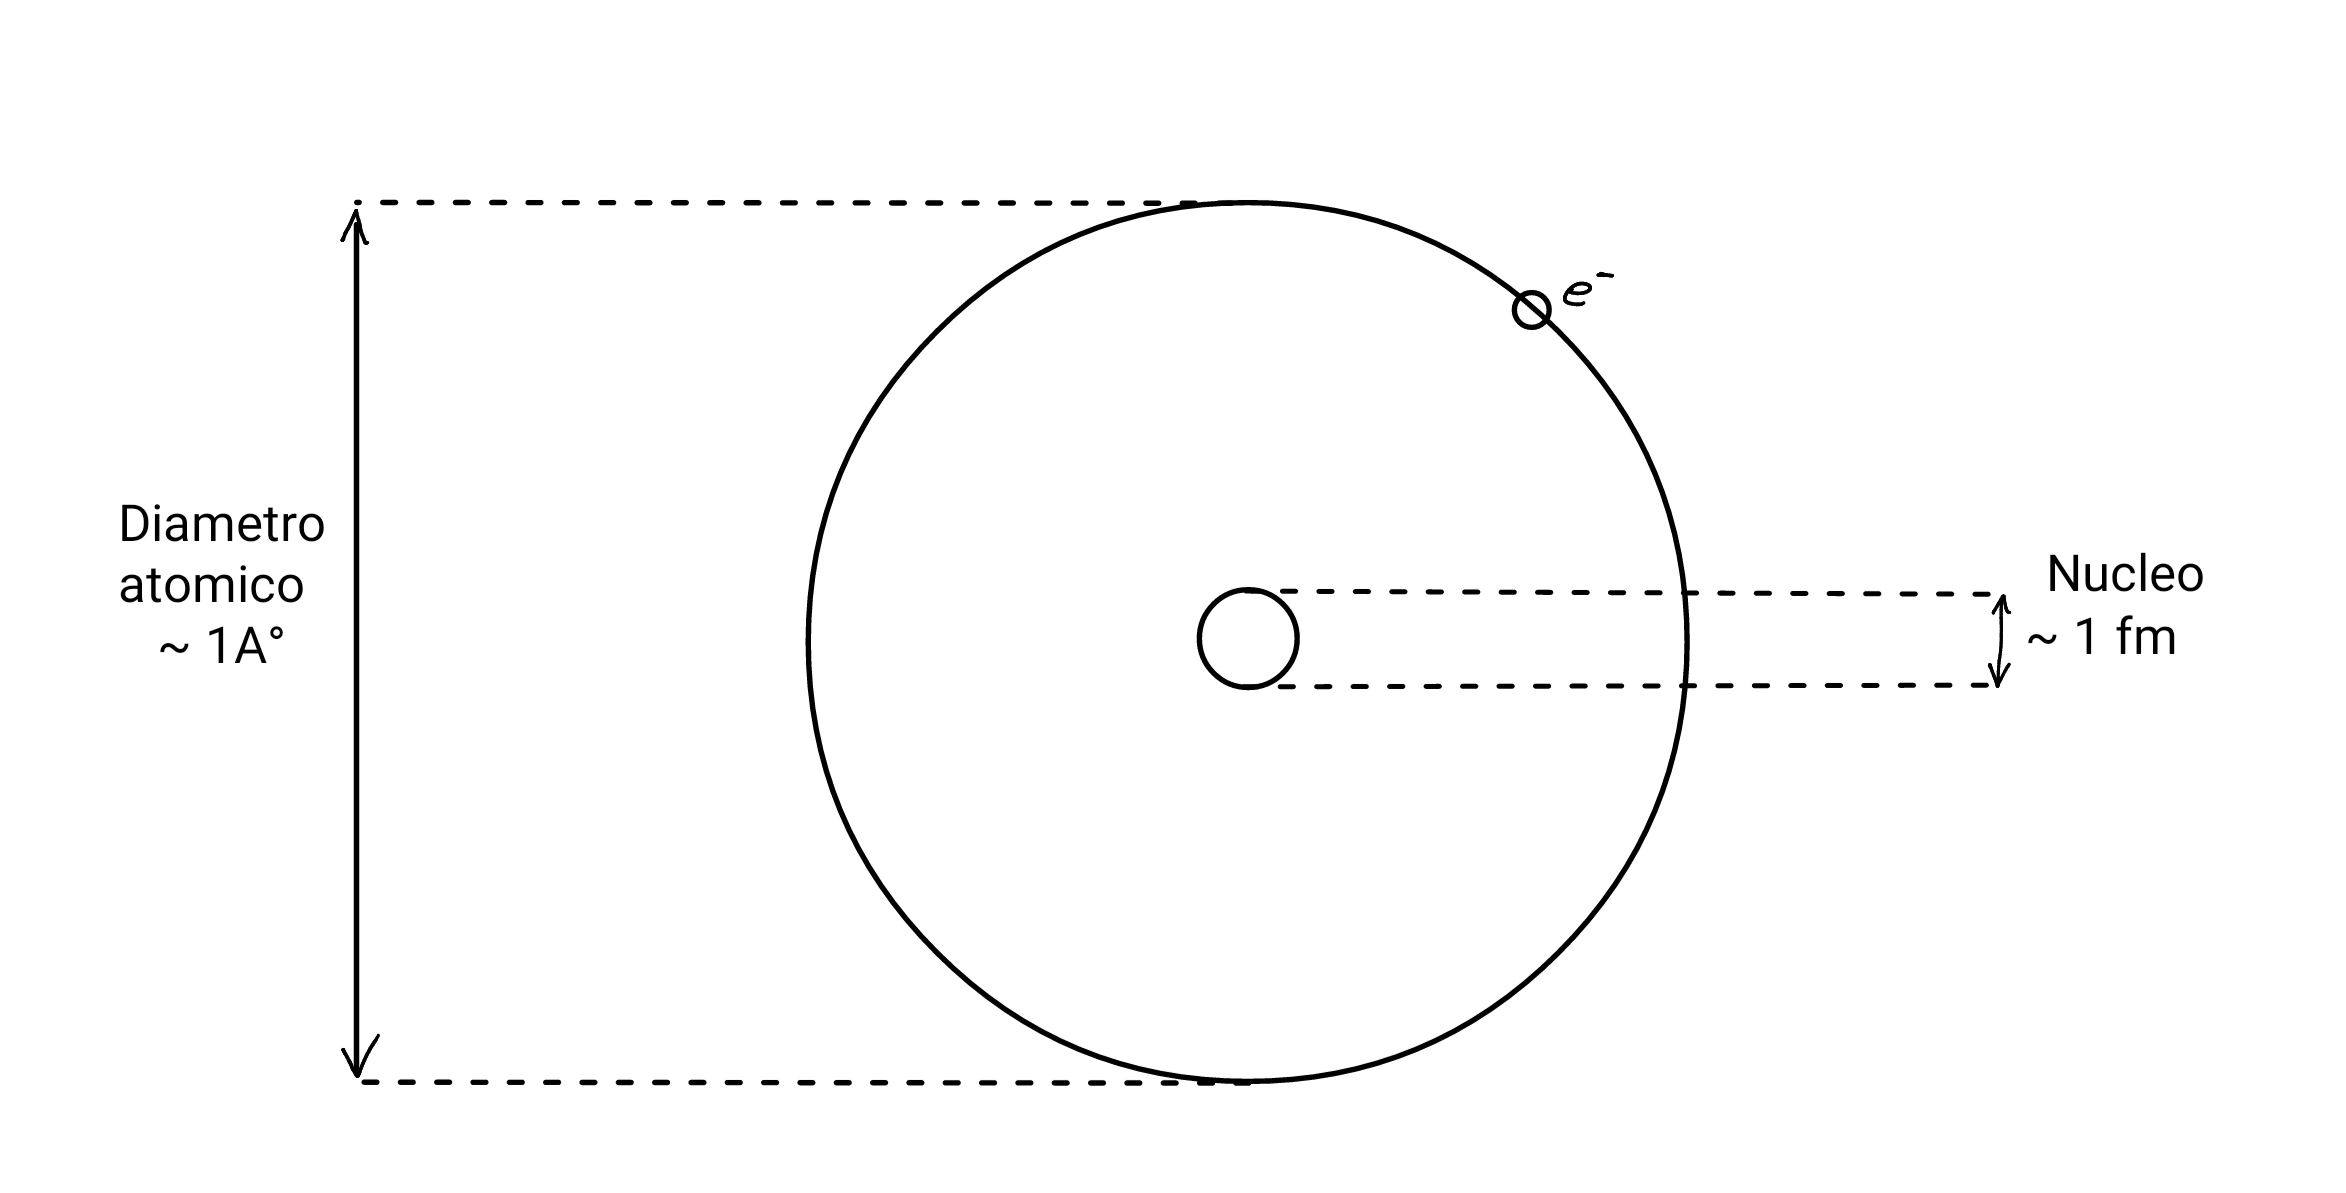
\includegraphics[width=0.6\textwidth]{immagini/dim-atomo.png}
	\caption{Dimensioni atomiche tipiche}
	\label{fig:atomo}
\end{figure}
Veniamo quindi agli scattering discussi, la situazione è modellizzata in Figura \ref{fig:rutherford}:
\begin{figure}[H]
	\centering
	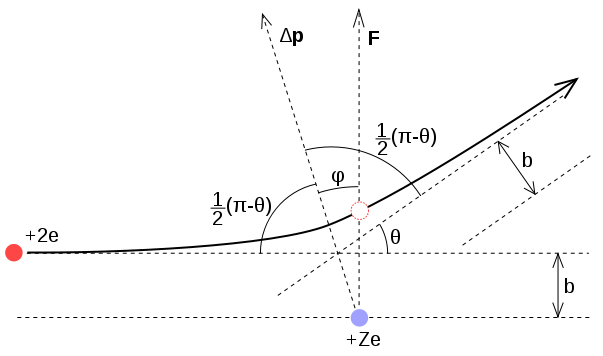
\includegraphics[width=0.8\textwidth]{immagini/rutherford.png}
	\caption{Schema dello scattering Rutherford.}
	\label{fig:rutherford}
\end{figure}
Per tutte le seguenti affermazioni viene considerto il centro scatterante come fisso (con massa molto maggiore del proiettile).
\paragraph{Interazione Columbiana.}
Inizialmente la particella ha una velocità $v_0$ che per la conservazione dell'energia e per simmetria deve essere uguale a quella finale $v_f$:
 \[
\left| \boldsymbol{v}_0 \right|  = \left| \boldsymbol{v}_f \right| 
.\] 
Si può trovare la variazione di impulso dopo interazione:
\[
	\Delta p = \left| \Delta \boldsymbol{p} \right| = \sqrt{\left( m \boldsymbol{v}_f - m \boldsymbol{v}_0 \right)^2} = m \sqrt{v_0^2 + v_0^2 -2v_0^2 \cos\left( \theta \right)} = 2m v_0 \sin\left( \frac{\theta}{2} \right)   
.\]
 
È utile anche ricordare la relazione che lega $\mu$ (angolo di riferimento che giace sul piano perpendicolare alla $\boldsymbol{v}_0$) all'elemento infinitesimo di sezione d'urto:
\[
d \sigma = b db d\mu
.\] 
Essendoci qua una simmetria sotto rotazioni attorno all'asse $\hat{v}_0$ possiamo integrare sull'angolo $\mu$ della relazione:
\[
d\sigma = 2 \pi b db
.\] 
Altra relazione differenziale che ci è utile adesso è: 
\[
\frac{\mbox{d} \sigma}{\mbox{d} \mu} = b db
.\] 
La sezione d'urto differenziale si può scrivere allora in funzione di $b\left( \theta \right)$ :
\[
	\frac{\mbox{d} \sigma}{\mbox{d} \Omega} = \frac{\mbox{d} \sigma}{\mbox{d}\mu \mbox{d}\cos\left( \theta \right) } = \frac{ b \mbox{d}b}{\mbox{d}\cos\left( \theta \right)} = - \frac{b \text{d}b}{ \sin\left( \theta \right) d \theta }  
.\]
Consideriamo adesso la variabile $\varphi$ nella Figura \ref{fig:rutherford} indice della posizione angolare dell'oggetto durante l'interazione, è definita appunto tra:
\[
\varphi_{\text{min}} = -\frac{\pi - \theta}{2} \le \varphi \le \frac{\pi -\theta}{2} = \varphi_{\text{max}}
.\] 
Possiaom giocarci la conservazione del momento angolare durante il processo sfruttando la variabile sopra definita come cordinata polare.
\[
	L_z = m \left( \boldsymbol{r \wedge \boldsymbol{v}}\right)_z = m \left[ \boldsymbol{r} \left( \dot{r} \hat{r} + r \dot{\varphi} \hat{\varphi}\right)\right]=
	mr^2\dot{\varphi}
.\] 
Quindi considerando anche il momento angolare iniziale abbiamo una prima relazione per parametrizzare il differenziale nel tempo:
\[
m v_0 b = m r^2 \frac{\mbox{d} \varphi}{\mbox{d} t} \quad \quad \implies \quad \quad dt = \frac{r^2}{b v_0} d\varphi
.\] 
Perche parametrizzare il tempo? Perche ci è utile per relazionare la variabile $b$ a $\theta$! Infatti la variazione di impulso calcolata sopra può essere scritta come:
\[
\left| \Delta \boldsymbol{p} \right| = \int_{-\infty}^{\infty} \left| \boldsymbol{F}_{\perp}\right| dt = 
\int_{-\infty}^{\infty} \left| \boldsymbol{F}\right| \cos\left( \varphi \right)  dt 
.\]
La forza citata è quella columbiana tra i due corpi:
\[
\left|\boldsymbol{F}\right| = \frac{zZe^2}{4 \pi \epsilon_0 r^2} 
.\] 
Mettiamo tutto nell'integrale (compreso il dt):
\[
	\left| \Delta \boldsymbol{p} \right| = \int_{\varphi_{\text{min}}}^{\varphi_{\text{max}}} \frac{zZe^2}{4 \pi \epsilon_0 b r^2} \frac{\cos\left( \varphi \right) }{b} \frac{r^2}{v_0} d \varphi 
	=  \frac{zZe^2}{2 \pi \epsilon_0 b v_0} \cos\left( \frac{\theta}{2} \right) 
.\] 
Senza mollare eliminiamo il $\left| \Delta \boldsymbol{p} \right|$ ricavato all'inizio:
\[
	2mv_0 \sin\left( \frac{\theta}{2} \right) = \frac{zZe^2}{2 \pi \epsilon_0 b v_0} \cos\left( \frac{\theta}{2} \right) 
.\] 
E le nostre fatiche vengono ripagate perche abbiamo la prima risposta:
\[
	b\left( \theta \right) = \frac{zZe^2}{4 \pi \epsilon_0 m  v_0^2} \cot\left( \frac{\theta}{2} \right) 
.\] 
È quindi possibile definire anche una minima distanza di urto centrale $d$ quando la cotangente è unitaria:
\[
	d = \frac{zZe^2}{4 \pi \epsilon_0 m  v_0^2} = \frac{zZ\left( \alpha \hbar c \right)}{T} \approx zZ \frac{1.44[\text{MeV}]}{T[\text{MeV}]} [\text{fm}]
	\quad \quad \implies \quad \quad b\left( \theta \right) = d \cot\left( \frac{\theta}{2} \right) 
.\] \label{eq:d-rutherford}
Apprezziamo la grandezza del risultato, siamo in grado di prevedere, note la carica e la massa del proiettile, la distanza ortogonale ($b$) tra i centri incidenti dal momento che scegliamo l'angolo di osservazione $\theta_0$ (o meglio, tutto ciò che arriva all'osservatore è partito da una posizione con parametro di impatto noto).\\
Si può infine trovare la sezione d'urto Rutherford differenziale come:
\[
	\frac{\mbox{d} \theta}{\mbox{d} \Omega} = -\frac{b db}{\sin\left( \theta \right) d \theta} =
	-\frac{b}{2 \cos\left( \frac{\theta}{2} \right) \sin\left( \frac{\theta}{2} \right)} \cdot \frac{d}{2}\left( \frac{d \left( \cot\left( \frac{\theta}{2} \right)\right)}{d \theta} \right) = 
	\ldots = \frac{d^2}{16 \sin^{4}\left( \frac{\theta}{2} \right) } 
.\] 

\paragraph{Interazione con sfera rigida}
In questo caso basta sfruttare alcune semplici considerazioni geometriche:
\[
	\frac{\text{d}\sigma}{\text{d} b} = 2 \pi b \quad \quad \text{ con } \quad b<R 
.\] 
A fare la differenza qua è la semplice definizione di $\theta$:
\[
	\frac{b}{R} = \sin\left( \frac{\pi - \theta}{2} \right) = \cos\left( \frac{\theta}{2} \right)  \implies b = R \cos\left( \frac{\theta}{2} \right) 
.\] 

% 2.b.21
\subsection[]{Calcolare la minima distanza fra le due particelle in uno scattering Rutherford.}
Definiamo $v_m$ come la velocità del proiettile nell'istante in cui ha raggiunto la distanza minima $x$. Sfruttando la conservazione dell'energia e del momento angolare si ottiene:
\[	
	\frac{1}{2}m v_0^2 = \frac{1}{2} m v_f^2 + \frac{zZe^2}{4 \pi \epsilon_0 x}\\
.\] 
\[
	mv_0b = m v_m x
.\]
Si ricava $v_m$ dalla seconda sostituendola nella prima, ne risulta una equazione del secondo grado per $x$:
 \[
	 x^2 - d \cdot x - b^2 = 0 \implies x = \frac{d}{2} \left( 1 + \frac{1}{\sin\left( \frac{\theta}{2} \right) } \right) 
.\] 
%2.b.22
\subsection[]{Calcolare l'energia minima affinché un protone possa avere una interazione forte "toccando" un nucleo di ${}^{12}C$ o di ${}^{28} Si$.}
È inanzitutto necessario per risolvere il problema di minimo considerare l'urto centrale: $b = 0$.\\ 
In tal caso l'angolo di scatternig è $\theta = \pi$ e $x = d$ dove $d$ è la distanza tra i nuclei aventi raggio:
\[
	R = \left( 1.25 A^{1 /3} + 2 \right) \text{fm} 
.\] 
L'energia minima è allora proprio l'energia potenziale necessaria ad arrivare alla distanza $d$:
 \[
	 E_{\text{min}} = \frac{zZe^2}{4 \pi \epsilon_0 \left( R_1 + R_2 \right) } 
.\] 
O molto più semplicemente (vista la fatica fatta in precedenza per \hyperref[eq:d-rutherford]{definire d}:
\[
	d = \left( R_1 + R_2 \right) \approx zZ\frac{1.44 [\text{MeV}]}{T[\text{Mev}] } [\text{fm}] \implies T = zZ\frac{1.44}{\left( R_1+R_2\right) } [\text{MeV}]
.\] 
Mettendo i numeri si ha:
\[
E_{\text{C}} \approx 1.4 \text{MeV} ,\quad \quad 
E_{\text{Si}} = 11.2 \text{MeV}
.\] 

%2.b.23
\subsection[]{Discutere le differenze tra lo scattering di Rutherford (particelle $\alpha$ su nuclei) e lo scattering di elettroni su bersaglio puntiforme.}
La differenza principale è che gli elettroni si muovono solitamente a velocità relativistiche, questo invalida i conti fatti prima. Nel caso discusso quindi è necessario tirare in ballo la sezione d'urto Mott.

%2.b.24
\subsection[]{Cercando i dati nelle apposite tabelle (reperibili sul web ) si indichino gli stati finali e si calcoli il Q-valore per i decadimenti delle seguenti specie instabili: ${}^8B, {}^{39}Ar, {}^{7}Be, {}^{64}Cu, {}^{76}Ge$. }
Per rispondere a questa domanda è necessario ricordarsi la natura dei \hyperref[sec:decadimenti]{Decadimenti} ed avere sottomano il Nuclear Wallet Card.
\paragraph{Isotopo del Boro}
\label{par:8B}
\[
	\ce{\ce{^{8}_{5}B_{3}} ->[\epsilon] \ce{^{8}_{4}\text{Be}_{4}} ->[\alpha] \ce{^{4}_{2}\text{He}^{2-}_{2}} } 
.\]
\[
	\Delta Q_{\epsilon} = \Delta_{A, Z} - \Delta_{A, Z-1} \approx 18 \text{ Mev} \quad \quad  
\]
\[
	\Delta Q_{\alpha} = ( 4m_u +  \Delta_{A,Z-1}) - \left( \Delta_{A-4, Z-2} + 4m_u + \Delta _{\alpha} \right) \approx 0.1 \text{ MeV}
.\] 
Quindi l'energia complessiva del processo è 
\[
	\Delta Q_{\epsilon}+ \Delta Q_{\alpha} \approx 18.1 \text{ MeV}.
\]
Notare che in questo caso particcolare i prodotti di decadimento $\alpha$ e $\ce{^{4}_{2}\text{He}^{2-}_{2}}$ hanno approssimativamente la stessa massa.
\paragraph{Isotopo dell'Argon}
\label{par:39Ar}
\[
	\ce{\ce{^{39}_{18}\text{Ar}_{21}}  ->[\beta^-] \ce{^{39}_{19}K_{20}}}
.\] 
\[
	\Delta Q_{\beta^-} = \Delta_{A,Z} - \Delta_{A, Z+1} = 0.57 \text{ MeV} 
.\] 
\paragraph{Isotopo del Berillio}%
\label{par:7Be}
\[
	\ce{\ce{^{7}_{4}\text{Be}_{3}} ->[\epsilon] \ce{^{7}_{3}\text{Li}_{4}} }
.\] 
\[
\Delta Q_{\epsilon} = \Delta_{A, Z} - \Delta_{A, Z-1} \approx 1.861 \text{ MeV}
.\] 
\paragraph{Isotopo del Rame}%
\label{par:64Cu}
Nelle tabelle sono indicate due possibilità, esaminiamo entrambe:
\[
	\ce{ \ce{^{64}_{30}\text{Zn}_{34}} <-[\beta^-][38.5 \%] \text{ } \ce{^{64}_{29}\text{Cu}_{35}} \text{ } ->[\epsilon][61.5\%] \ce{^{64}_{28}\text{Ni}_{36}} }
.\] 
Senza essere ripetitivi (stesse cose viste sopra) si riportano i risultati:
\[
\Delta Q_{\epsilon} = 1.67 \text{ MeV}
.\] 
\[
\Delta Q_{\beta^-} = 0.68 \text{ MeV}
.\] 

\paragraph{Isotopo del Germanio}%
\label{par:76Ge}
\[
	\ce{^{76}_{32}\text{Ge}_{44}} \implies \tau_{1 /2} \sim 2 \cdot 10^{21} 
.\]
Al gran sasso si studia il decadimento $\beta^- \beta^-$ di Questo isotopo (nome in codice GERDA).
\paragraph{Nota:} I conti della domanda sono stati fatti senza calcolatore per allenamento, siete fortemente invitati a fare lo stesso e riportare gli errori a chi ha accesso al source code.

% 2.b.25
\subsection[]{Cercando i dati nelle apposite tabelle (reperibili sul web) si trovino i Q-valori per le reazioni 
\begin{enumerate}
	\item $n + {}^{154}Gd \implies \gamma + {}^{155}Gd$ 
	\item $n + {}^{155}Gd \implies \gamma + {}^{156}Gd$
\end{enumerate}
}
\[
	\Delta Q_1 = \left( m_n + 154 m_u + \Delta_{154, 64} \right) - \left( 155m_u + \Delta_{154, 64 } \right) \approx 6.43 \text{ MeV} 
.\]
\[
	\Delta Q_2 = \ldots \approx m_{n} - m_{u} + \Delta_{155,64}-\Delta_{156,64} \approx 7.4 \text{ MeV} 
.\] 

% 2.b.26
\subsection[]{Dimostrare che $\frac{d^3 p  }{2E}$ è un invariante relativistico effettuando esplicitamente la trasformazione di Lorentz (si consideri il boost lungo un asse, per esempio l'asse x)}
Facciamo questo boot lungo x:
\begin{align*}
	\frac{\mbox{d}^3 \boldsymbol{P}'}{2E'}  =& \frac{dP'_x dP'_y dP'_z}{2Ex'} = \\
	=& \frac{\gamma d\left( P_x + \beta E \right)dP_y dP_z }{2 \gamma\left( E + \beta P_x \right)} = \\
	=& \frac{ \left[ dP_x + \beta d \sqrt{P_x^2 + m^2}\right]dP_y dP_z  }{2\left( E + \beta P_x \right) } = \\ 
	=& \frac{\left( dP_x + \beta\frac{2P_x dP_x}{2\sqrt{P_x^2 + m^2} } \right)dP_y dP_z }{2\left( E + \beta P_x \right)} = \\
	= & \frac{\mbox{d}^3 \boldsymbol{P}}{2E}
.\end{align*}

% 2.b.27
\subsection[]{Dimostrare che 
\[
d^{4}P \delta\left( P^2-m^2 \right) \theta\left( P_0 \right) = \frac{d^3 \boldsymbol{P} }{2E}
\]
e sfruttare questo risultato per semplificare la scrittura dell’elemento infinitesimo dello spazio dei 4-impulsi di N particelle emergenti dopo la collisione di due particelle (oppure dopo il decadimento di una particella).}
È sufficiente rimembrare una delle proprietà della $\delta$:
\[
	\delta\left( f\left( x \right)  \right) = \sum_{j} \frac{\delta\left( x-x_j \right) }{\left| \left[ f'\left( x \right)  \right]_{x = x_j} \right| }
.\] 
Da inserire opportunamente nella espressione a sinistra dell'uguale nella richiesta: dobbiamo ricordare che $P$ è in realtà un quadrivettore.
\begin{align*}
	d^{4}P \cdot \delta\left( P^2-m^2 \right) \theta\left( P_0 \right) =& d^4P\cdot  \delta\left(\boldsymbol{P}^2 - P_0^2 - m^2 \right) \theta\left( P_0 \right)  = \\
	=& d^4 P \cdot  \theta\left( P_0 \right) \left[ \frac{\delta\left( P_0 - E \right) }{\left| \left[ 2P_0 \right]_{P_0 = E} \right| } + 
		\frac{\delta\left( P_0 + E \right) }{\left| \left[ 2P_0 \right]_{P_0 = -E}  \right| } \right] =\\
		=& d^4P \frac{\delta\left( P_0 - E \right)}{2E} = \frac{d^3 \boldsymbol{P}}{2E}   
.\end{align*}
\paragraph{Nota:}%
Stiamo parlando di distribuzioni, la notazione leggera utilizzata nasconde significati matematici profondi e non scontati (vedi corso di metodi matematici per la fisica II).

% 2.b.28
\subsection[]{Dimostrare che nel centro di massa l’elemento infinitesimo dello spazio dei 4-impulsi, nel caso di 2 sole particelle nello stato finale, si scrive come $\frac{|\boldsymbol{p_{cm}}}{4\sqrt{s}} d\Omega_{cm}.$}
Ricordiamo la forma dell'elemento infinitesimo dello spazio delle fasi:
\[
	dL_p = \left[ d^4P_1 \cdot \delta\left( P_{0,1}^2 - \boldsymbol{P}_1^2 - m_1^2 \right) \cdot \theta\left( P_{0,1} \right) \right] \cdot \ldots 
	\left[ \cdot d^4P_n \cdot \delta\left( P_{0,n}^2 - \boldsymbol{P}_n^2 - m_n^2 \right) \cdot \theta\left( P_{0,n} \right) \right] \cdot 
	\delta^4\left(  P_{in}-\sum_{i}P_i  \right) 
.\]
Che utilizzando la risposta alla domanda precedente si riscrive come:
\[
dL_p = \frac{\mbox{d}^3 \boldsymbol{P}_1}{2E_1} \ldots \frac{\mbox{d}^3 \boldsymbol{P}_n}{2E_n} \delta^4\left( P_{in}-\sum_{i}P_i \right) 
.\] 
Decisamente più carino.\\
Se si hanno due prodotti definiamo le loro masse come $m_1$ e  $m_2$, l'energia del centro di massa $\sqrt{s}$ e ricordiamo che il 3-impulso totale nel centro di massa è nullo. L'elemento infinitesimo $dL_p$ si scrive come:
\begin{align*}
	dL_p =& \frac{d^3 \boldsymbol{P}_1}{2E_1} \frac{d^3 \boldsymbol{P}_2}{2E_2} \cdot \delta^4\left(P_{\text{in}} - P_1 - P_2 \right) = \\ 
	= & \frac{d^3 \boldsymbol{P}_1}{2E_1} \frac{d^3 \boldsymbol{P}_2}{2E_2} \cdot \delta\left( \sqrt{s}-E_1-E_2\right) \cdot 
	\delta^3\left( \boldsymbol{0} + \boldsymbol{P}_1 + \boldsymbol{P}_2 \right) = \\
	= & \frac{ d \boldsymbol{P}_1 }{4E_1E_2} \cdot \delta\left( \sqrt{s}-E_1-E_2\right)   
\end{align*}
Passando in cordinate spefiche:
\[
	dL_p = \frac{P_1^2 dP_1 d \Omega_1 }{4E_1E_2} \cdot \delta\left( \sqrt{s} -E_1-E_2  \right) 
.\]
Possiamo adesso sfruttare il fatto che nel centro di massa l'impulso totale è nullo, chiamiamo $P_{\text{cm}}$ l'impulso della particella singola (le due particelle hanno in modulo lo stesso impulso in questo sistema $\left| \boldsymbol{P}_1 \right| = \left| \boldsymbol{P}_2 \right| = P_{\text{cm}}$):
\[
	\sqrt{s}= \sqrt{P_{\text{cm}}^2 + m_1^2} + \sqrt{ P_{\text{cm}}^2 + m_2^2} 
.\] 
Che può essere risolta ( Hint: servono due elevazioni al quadrato) per $P_{\text{cm}}$ :
\[
	P_{\text{cm}} = \sqrt{\frac{\left( s - \left( m_1+m_2 \right)^2 \right) \left( s - \left( m_1 - m_2 \right)^2 \right)}{4s}} 
.\]
Non esplicitiamo $P_{\text{cm}}$ nei calcoli a seguire, è bene però sappere che può essere scritto in funzione di variabili più "comuni". La relazione sopra sarà sfruttata al secondo passaggio del seguente calcolo.
\begin{align*}
	dL_p =& \frac{P_1^2 dP_1 d \Omega_1}{4E_1E_2} \cdot \delta\left( \sqrt{s} - \sqrt{P_1^2 + m_1^2} - \sqrt{P_2^2 + m_2^2}  \right) \\
	=& \frac{P_1^2 dP_1 d \Omega_1}{4E_1E_2} \cdot 
	\frac{\delta\left(P_1-P_{\text{cm}}\right)}{\left|\left[\frac{\mbox{d}}{\mbox{d}P_1}\left(\sqrt{s}-\sqrt{P_1^2+m_1^2}-\sqrt{P_1^2+m_2^2}\right)\right]_{P_1=P_{\text{cm}}}\right|} = \\
	=& \frac{P_1^2 dP_1 d \Omega_1}{4E_1E_2} \cdot \frac{ \delta \left( P_1-P_{\text{cm}} \right) }{ \left| \left[ \frac{P_1}{E_1}+\frac{P_1}{E_2} \right]_{P_1=P_{\text{cm}}} \right|}=\\
	=& \frac{P_1^2 dP_1 d \Omega_1}{4E_1E_2} \cdot \frac{\delta\left(P_1-P_{\text{cm}}\right)}{P_{\text{cm}} \frac{E_1 + E_2}{E_1E_2}} = \\
	=& \frac{P_{\text{cm}} }{4\sqrt{s}} d\Omega_{1}
\end{align*}
Noto l'impulso delle particelle nel centro di massa (o, se si vuole, $\sqrt{s}, m_1, m_2$) si ha che l'elemento infinitesimo dello spazio delle fasi dei due prodotti dipende solo dall'angolo solido di un prodotto (che in caso di isotropia spaziale come qua è l'opposto di $\Omega_2$). Questo è molto utile per la sezione d'urto differenziale ad esempio.
\[
	\frac{\mbox{d} \sigma}{\mbox{d} \Omega_1} = f_{\text{urto}}\left( \Omega_1 \right) \frac{P_{\text{cm}}}{4\sqrt{s} }
.\] 

% 2.b.29
\subsection[]{Nel caso di 3 particelle nello stato finale di una reazione, dimostrare che fra il quadrato della massa invariante di due di esse e l'energia della terza (nel centro di massa) sussite una relazione lineare.}
Prendiamo la massa invariante citata $\sqrt{s_{12}}$ e l'energia della restante paticella come $E_3$, con ovvio significato dei simboli si ha (definizione di massa invariante):
\[
	s_{12} = \left( P_1 + P_2 \right)^2
.\] 
Che per la conservazione dell'energia e dell'impulso si può scrivere come:
\[
	s_{12} = \left( P_{\text{in}} - P_3 \right)^2 = P_{\text{in}}^2 + P_3^2 - 2 P_{\text{in}}P_3 =s + m_3^2 - 2 \sqrt{s}E_3 
.\] 
Ecco la relazione lineare.

% 2.b.30
\subsection[]{Come si trasforma una funzione di distribuzione del 3-impulso 
\[
	f\left( \boldsymbol{p} \right)d^3 \boldsymbol{p}
\]
di una particella per una trasformazione di Lorentz?}
Premessa: misurare in un sistema la funzione di distribuzione del 3-impulso significa misurare il numero di eventi dn nell'elemento di volume nello spazio degli impulsi $dn = f\left( \boldsymbol{P} \right) d^3 \boldsymbol{P}$. È inoltre naturale che il numero di eventi registrati deve essere lo stesso in ogni sistema di riferimento 
\[
dn = f\left( \boldsymbol{P} \right) d^3 \boldsymbol{P} =  f\left( \boldsymbol{P}' \right) d^3 \boldsymbol{P}' = dn'
\]
Abbiamo dimostrato anche che 
\[
\frac{d^3 \boldsymbol{P}}{2E} 
.\] 
è un invariante relativistico, quindi si può concludere:
\[
	\frac{E}{E} f\left( \boldsymbol{P} \right) d^3 \boldsymbol{P} = \frac{E'}{E'} f\left( \boldsymbol{P}' \right) d^3 \boldsymbol{P}' \quad \implies \quad 
	f\left( \boldsymbol{P}' \right) = \frac{E}{E'} f\left( \boldsymbol{P} \right) 
.\] 

% 2.b.31
\subsection[]{Come si trasforma una funzione di distribuzione nello spazio delle fasi 
\[
	f\left(\boldsymbol{p},\boldsymbol{r}\right)d^3 \boldsymbol{p} \ d^3 \boldsymbol{r} 
\]
di una particella per una trasformazione di Lorentz?}
È necessario notare che anche qua il numero di eventi $dn$ nel volume infinitesimo dello spazio delle fasi si deve conservare come sopra, ragionando quindi allo stesso modo si trova la legge di trasformazione richiesta.\\
Mettiamoci per utilità nel sistema in cui la particella è a riposo e consideriamo un boost lungo uno dei 3 assi di riferimento, possiamo sfruttare la contrazione delle lunghezze
\[
\text{d}^3 \boldsymbol{r}' =\frac{\text{d}^3\boldsymbol{r}}{\gamma} =  \frac{\text{d}^3\boldsymbol{r}}{E'} mc^2 = \frac{\text{d}^3\boldsymbol{r}}{E'} E
.\] 
Quindi $Ed^3 \boldsymbol{r}$ è un invariante relativistico. Avendo trovato che anche $d^3 \boldsymbol{P} / E$ è invariante si ha che
\begin{align*}
	dn = f\left( \boldsymbol{P}, \boldsymbol{r} \right) \text{d}^3 \boldsymbol{P} \text{d}^3 \boldsymbol{r} =  f\left( \boldsymbol{P}', \boldsymbol{r}' \right) 
	\text{d}^3 \boldsymbol{P}' \text{d}^3 \boldsymbol{r}' = dn' & \quad \quad
	\text{Invarianza del numero di eventi} \\
	\frac{\text{d}^3 \boldsymbol{P}}{E} E \text{d}^3 \boldsymbol{r} =
	\frac{\text{d}^3 \boldsymbol{P}'}{E'} E' \text{d}^3 \boldsymbol{r}' & \quad \quad 
	\text{Invarianti trovati sopra}
.\end{align*}
Dalle quali deriva l'invarianza di $f\left( \boldsymbol{P}, \boldsymbol{r} \right)$.

% 2.b.32
\subsection[]{Dimostrare che se la probabilità di decadimento di una particella per unità di tempo non dipende dal tempo, la probabilità di trovare la particella non decaduta al tempo t segue una legge esponenziale.}
Sia $S\left( t \right) $ la probabilità di trovare la particella al tempo $t$, considerando la invece la probabilità $P\left( t \right)$ di decadere dopo l'unità di tempo $dt$ si ha (per ipotesi):
 \[
	 \frac{P\left( dt \right)}{dt}= \frac{1}{\tau} \text{ (costante)} \implies  S\left( dt \right) = 1 - \frac{dt}{\tau}
.\] 
Quindi all'istante $t + dt$ si ha (per le regole delle probabilità combinate):
\[
	S\left( t + dt \right) = S\left( t \right) S\left( dt \right) = S\left( t \right) \left( 1 - \frac{dt}{\tau} \right) 
.\] 
Che ha come soluzione proprio un esponenziale (vedi \hyperref[sec:2.b.5]{Domanda 2.b.5}):
\[
	S\left( t \right) = e^{- t / \tau}
.\] 

% 2.b.33
\subsection[]{ Dire quali fra le seguenti particelle sono soggette ad interazioni forti: $ p, \overline{p} $, $\pi^{+}, \pi^{-}, \mu^{+}, \mu^{-}, e^{+}$, $e^{-}$, $\alpha,$ Nucleo di Azoto, $\nu, \overline{\nu}$ }
\label{sec:2.b.33}
Solo gli adroni (composti da Quark) possono fare interazione forte, quindi la risposta è: $p$ , $\overline{p}$ , $\pi^{+}$ , $\pi^{-}$ , $\alpha$ , Nucleo di Azoto.

\subsection[]{Pioni neutri, di energia E nel sistema del laboratorio, decadono in due fotoni. La distribuzione è isotropa ne centro di massa. Si calcoli la distribuzione dell’energia di uno dei due fotoni nel laboratorio e gli angoli, rispetto alla direzione di volo del pione, dei due fotoni nel sistema del laboratorio in funzione dell’angolo nel sistema del centro di massa.}
\begin{figure}[H]
	\centering
	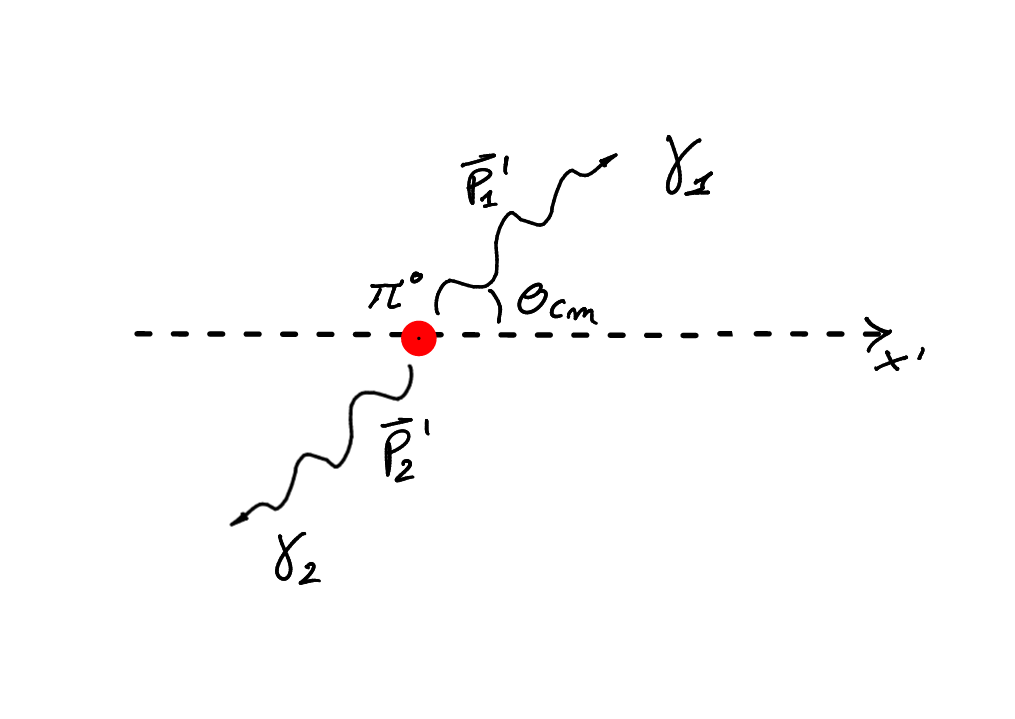
\includegraphics[width=0.35\textwidth]{immagini/decadimento-pi1.png}
	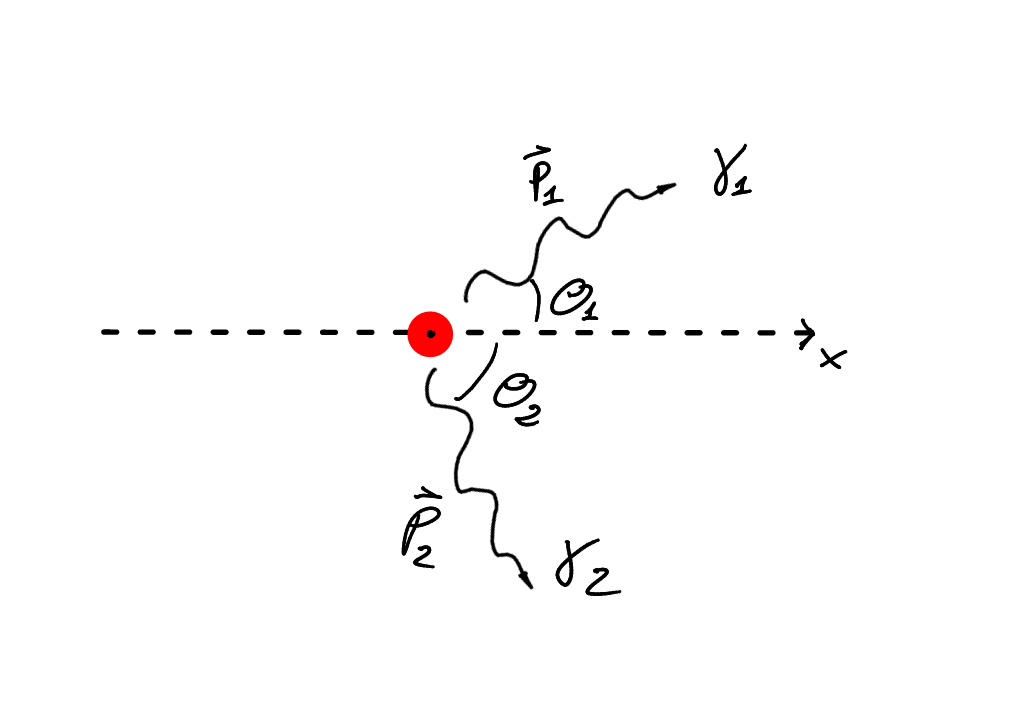
\includegraphics[width=0.35\textwidth]{immagini/decadimento-pi2.png}
	\caption{Decadimento del $\pi^0$ in due fotoni: a sinistra nel centro di massa e a destra nel sistema del laboratorio.}
	\label{fig:Decadimento del Pione in fotoni.}
\end{figure}
Fissando idee e notazione come in Figura \ref{fig:Decadimento del Pione in fotoni.} procediamo al calcolo richiesto.
\[
	\ce{\ce{\pi} -> \ce{\gamma} + \ce{\gamma}}
.\] 
La massa del $\pi^0$ è 134.96 MeV, assumiamo che nel laboratorio questo si muova con velocità $\beta$ nell'istante precedente al decadimento. Nel sistema del $\pi^0$ si ha:
 \[
P_1' = \frac{m}{2} \cdot 
\begin{pmatrix}
	1 \\
	\cos\left( \theta_{\text{cm}} \right) \\
	\sin\left( \theta_{\text{cm}} \right) \\
	0
\end{pmatrix} \quad \quad \quad 
P_2' = \frac{m}{2}\cdot 
\begin{pmatrix} 
	1 \\
	-\cos\left( \theta_{\text{cm}}\right) \\
	- \sin\left( \theta_{\text{cm}} \right) \\
	0
\end{pmatrix} 
.\] 
Essendo inoltre la distrubuzione di prodotti isotropa nel centro di massa possiamo scrivere:
\[
	\frac{\text{d} \Gamma}{\text{d}\Omega_{\text{cm}}} = \frac{\Gamma}{4 \pi} \quad \quad \implies \quad \quad 
	\frac{\text{d} \Gamma}{\text{d}\cos\left( \theta_{\text{cm}} \right) } = \frac{\Gamma}{2}
.\] \label{eq:isotropia}
Nel laboratorio si ha invece:
\[
P_1 = E_1 \cdot 
\begin{pmatrix}
	1 \\
	\cos\left( \theta_1 \right) \\
	\sin\left( \theta_1 \right) \\
	0
\end{pmatrix} \quad \quad \quad 
P_2 = E_2\cdot
\begin{pmatrix} 
	1 \\
	\cos\left( \theta_2 \right) \\
	 \sin\left( \theta_2 \right) \\
	0
\end{pmatrix} 
.\] 
È possibile limitare le energie dei prodotti nel laboratorio tramite una trasformazione di Lorentz:
\begin{align*}
	E_1=&\gamma\frac{m}{2}\left(1+\beta\cos\left(\theta_{\text{cm}}\right)\right)&
		\quad E_2=&\gamma\frac{m}{2}\left(1-\beta\cos\left(\theta_{\text{cm}}\right)\right)\\
	P_{1,x} = E_1 \cos\left( \theta_{1} \right) =& \gamma \frac{m}{2} \left( \beta + \cos \left(\theta_{\text{cm}} \right) \right)   &
		\quad P_{2,x} = E_2 \cos\left( \theta_2 \right) =& \gamma \frac{m}{2} \left( \beta - \cos\left( \theta_{\text{cm}} \right)  \right) \\ 
	P_{1,y} = E_1 \sin\left( \theta_1 \right) =& \frac{m}{2}\sin\left( \theta_{\text{cm}}\right) &
		\quad P_{2, y} =E_2\sin\left( \theta_2 \right) =& - \frac{m}{2} \sin\left( \theta_{\text{cm}}\right) 
.\end{align*}
Guardando alla prima colonna facendo variare il $\cos\left( \theta_{\text{cm}} \right) $ con la fantasia è facile vedere che:
\[
	\gamma \frac{m}{2}\left( 1 - \beta \right) \le E_1 \le \gamma \frac{m}{2} \left( 1 + \beta \right) 
.\] 
Possiamo adesso calcolarci come è distribuita l'energia $E_1$ (della particella 1 nel laboratorio):
\[
	\frac{\mbox{d} \Gamma}{\mbox{d} E_1} = 
	\frac{\mbox{d} \Gamma}{\mbox{d} \cos\left( \theta_{\text{cm}} \right) } \frac{\mbox{d} \cos\left( \theta_{\text{cm}} \right) }{\mbox{d} E_1} =
	\frac{\Gamma}{2} \frac{2}{m \gamma \beta} = \frac{\Gamma}{m \gamma \beta}
.\] 
La distribuzione è quindi piatta (non dipende da $E_1$) e ben normalizzata se integrata nei limiti di $E_1$.\\
Per quanto riguarda la seconda richiesta procediamo calcolando la distribuzione angolare di uno dei fotoni.
Per farlo possiamo sfruttare ancora le trasformazioni di Lorentz di cui sopra isolando gli angoli nel laboratorio (essenzialmente la risposta al quesito è questa):
\begin{align*}
	\cos\left(\theta_1\right)=&\frac{P_{1,x}}{E_1}=\frac{\beta+\cos\left(\theta_{\text{cm}}\right)}{1+\beta\cos\left(\theta_{\text{cm}}\right)}\quad&  
	\cos\left(\theta_2\right)=&\frac{P_{2,x}}{E_2}=\frac{\beta-\cos\left(\theta_{\text{cm}}\right)}{1-\beta\cos\left(\theta_{\text{cm}}\right)} \\  
	\sin\left(\theta_1\right)=&\frac{P_{1,y}}{E_1}=\frac{\sin\left(\theta_{\text{cm}}\right)}{\gamma\left(1+\beta\cos\left(\theta_{\text{cm}}\right)\right)}\quad&
	\sin\left(\theta_2\right)=&\frac{P_{1,y}}{E_2}=\frac{-\sin\left(\theta_{\text{cm}}\right)}{\gamma\left(1-\beta\cos\left(\theta_{\text{cm}}\right)\right)}
.\end{align*}
Dalla prima in alto si ricava la cosa che ci serve: $\cos\left( \theta_{\text{cm}} \right)$ in funzione di $\cos\left( \theta_1 \right)$:
\[
	\cos\left( \theta_{\text{cm}} \right) = \frac{-\beta + \cos\left( \theta_1 \right) }{1 - \beta\cos\left( \theta_1 \right) }
.\] 
Sfruttiamo adesso l'isotropia nel centro di massa:
\begin{align*}
	\frac{\text{d}\Gamma}{\text{d}\cos\left( \theta_{1} \right) } =&
	\frac{\mbox{d}\Gamma}{\mbox{d}\cos\left(\theta_{\text{cm}}\right)}\frac{\mbox{d}\cos\left(\theta_{\text{cm}}\right)}{\mbox{d}\cos\left(\theta_1\right)}=\\
	=&\frac{\Gamma}{2}\frac{1-\beta\cos\left(\theta_1\right)-(-\beta)(-\beta+\cos(\theta_1))}{\left(1-\beta\cos(\theta_1)\right)^2} =\\
	=& \frac{\Gamma}{2}\frac{1-\beta^2}{\left( 1-\beta\cos\left(\theta_1\right)\right)^2}=\\
	=&\frac{\Gamma}{2\gamma^2}\frac{1}{\left(1-\beta\cos(\theta_1)\right)^2}
.\end{align*}
Nell'ultima equazione si evidenzia come siano prediletti angoli piccoli (funzione crescente al tendere di $\ce{\ce{\theta_1} -> 0 }$).\\
Infine possiamo dire qualcosa in più sulla differenza degli angoli nel laboratorio, nonchè "l'apertura" del cono formato dalla direzione dei due fotoni nel lab:
\[
	\sin\left( \theta_1-\theta_2 \right) = \sin\left( \theta_1 \right) \cos\left( \theta_2 \right) -\sin\left( \theta_2 \right) \cos\left( \theta_1 \right) =
	\frac{2 \beta\sin\left( \theta_{\text{cm}} \right) }{\gamma\left( 1-\beta^2\cos^2\left(\theta_{\text{cm}}\right)\right) }
.\]
Questa funzione vista la dipendenza da $\beta$ fa cose diverse a seconda della velocità del $\pi^0$. 

%2.b.35
\subsection[]{ Calcolare la funzione di distribuzione in energia ed in angolo nel sistema del laboratorio di un fascio di neutrini o di muoni prodotto nel decadimento di pioni carichi di energia 14 GeV.}
\[
	\ce{\ce{\pi^+} -> \ce{\mu^+} + \ce{\nu_{\mu}}}
.\] 
Con  $m_{\pi^+} = 139.57$, $m_{\mu}=105.66$ e $m_{\nu}=0$. Se il pione ha energia 14 GeV allora avrà
\[
\gamma = \frac{E}{mc^2} = 100 \implies \beta \approx 0.99994
.\] 
Mettiamoci nel sistema del $\pi^+$, i 4-vettori energia-impulso dei prodotti sono:
\[
P'_{\mu} =  
\begin{pmatrix}
	\sqrt{P_{\text{cm}}^2+m_{\mu}^2}  \\
	P_{\text{cm}}\cos\left( \theta_{\text{cm}} \right) \\
	P_{\text{cm}}\sin\left( \theta_{\text{cm}} \right) \\
	0
\end{pmatrix} \quad \quad \quad 
P'_{\nu} = 
\begin{pmatrix} 
	P_{\text{cm}} \\
	-P_{\text{cm}}\cos\left( \theta_{\text{cm}} \right) \\
	-P_{\text{cm}}\sin\left( \theta_{\text{cm}} \right) \\
	0
\end{pmatrix} 
.\] 
Applichiamo la conservazione dell'energia nel centro di massa per esprimere $P_{\text{cm}}$ in funzione delle sole masse invarianti:
\[
	m_{\pi} = E'_{\mu} + E'_{\nu} =
	\sqrt{P_{\text{cm}}^2 + m_{\mu}^2} + P_{\text{cm}} \quad \implies
	\quad P_{\text{cm}} = \frac{m_{\pi}^2 - m_{\mu}^2}{2m_{\pi}} \approx 30\text{ Mev}
.\]
Visto che il pione ha spin nullo si ha anche qua l'isotropia dei prodott, quindi il \hyperref[eq:isotropia]{risultato} della domanda precedente su $\frac{\text{d}\Gamma}{\text{d}\Omega}$.
Trasformiamo allora per l'energia del neutrino nel laboratorio:
\[
	E_{\nu}^{\text{lab}}=\gamma P_{\text{cm}} \left(1-\beta\cos\left( \theta_{\text{cm}}\right)\right) 
.\] 
In cui si trovano di nuovo limiti inferiori essendoci $\cos\left( \theta_{\text{cm}} \right) $ di mezzo:
\[
	0 \approx \gamma P_{\text{cm}}\left( 1-\beta \right) \le E_{\nu}^{\text{lab}}\le \gamma P_{\text{cm}}\left( 1+\beta \right) \approx 6.2 \text{ GeV}
.\] 
Abbiamo tutte le carte per calcolare la distribuzione del neutrino:
\[
	\frac{\mbox{d} \Gamma}{\mbox{d} E_{\nu}^{lab}} = 
	\frac{\mbox{d} \Gamma}{\text{d}\cos\left( \theta_{\text{cm}} \right) } \frac{\text{d}\cos\left( \theta_{\text{cm}} \right) }{\mbox{d} E_{\nu}^{lab}} =
	= \frac{\Gamma}{2}\frac{1}{P_{\text{cm}}\beta \gamma}
.\] 
Analogamente si può fare per il $\mu$:
\[
	E_{\mu}^{\text{lab}}=\gamma\left( \sqrt{P_{\text{cm}}^2+m_{\mu}} + \beta P_{\text{cm}}\cos\left( \theta_{\text{cm}}\right)\right)
.\] 
\[
	7.8 \text{ GeV} \approx \gamma\left( \sqrt{P_{\text{cm}}^2 + m_{cm}^2} - \beta P_{\text{cm}} \right) \le E_{\mu}^{\text{lab}} \le 
	\gamma\left( \sqrt{P_{\text{cm}}^2 + m_{cm}^2} + \beta P_{\text{cm}} \right)  \approx 14 \text{ GeV}
.\] 
\[
\frac{\mbox{d} \Gamma}{\mbox{d} E_{\mu}^{\text{lab}}} = \frac{\Gamma}{2}\frac{1}{P_{\text{cm}}\beta \gamma}
.\] 

%2.b.36
\subsection[]{ Qual e' l'andamento delle masse nucleari a parità di A in funzione di Z?}
I nuclei isobari (a parità di A) hanno una massa con andamento quadratico in Z:
\begin{align*}
	M_{A,Z}^{\text{atomo}} =& ZM_H^{\text{atomo}} + Nm_n - B_{A,Z} =\\
	=&ZM_H^{\text{atomo}}+\left(A-Z\right)m_u-\text{cost}\left(A\right)-a_s\frac{Z^2}{A^{1/3}}-a_{\text{sym}}\frac{\left(Z-N\right)^2}{A}-\delta_{\text{pair}}
.\end{align*}

% 2.b.37
\subsection[]{ Dimostrare che in un tipico decadimento $\alpha$, la particella $\alpha$ emerge con circa il 98\% dell'energia disponibile.}
In un decadimento $\alpha$ si ha:
\[
\ce{\ce{^{A}_{Z}X_{N}} -> \ce{^{A-4}_{Z-2}Y_{N-2}} + \alpha}
.\]
\paragraph{Metodo Complicato}%

In decadimento tipico di questi si ha anche che $A\gg 4$, ,$Z\gg 2$. Inoltre $B\left( 4,2 \right) = 28.3$ MeV. Forti di queste informazioni immagineremo un piano $A,Z$ pensando queste come variabili indipendenti per poter fare alcune approssimazioni in seguito. Calcoliamo intanto il Q-valore.\\
Nel calcolo del $Q$-valore del processo utilizziamo la massa dell'atomo scritta come:
\[
M_{A,Z} = ZM_H + N m_n - B_{A,Z} 
.\] 
Notiamo che, conservandosi il numero di protoni e neutroni il $Q$-valore si riduce alla differenza delle Biniding Energy $B$ con particolare attenzione ad i segni nella \hyperref[eq:Q-valore]{Definizione di $Q$}:
 \[
	 Q_{\alpha} = B\left( A-4,Z-2 \right) + B\left( 4,2 \right) - B\left( A,Z \right) 
.\] 
Ragionando sempre in termini di $A,Z$ generigi sfruttiamo le ipotesi $A\gg 4$ e $Z\gg 2$ per sviluppare il termine $B\left( A-4,Z-2 \right) $ attorno al punto $\left[ A , Z \right]$:
\[
	B\left( A-4,Z-2 \right) \approx B\left( A, Z \right) - 4 \frac{\partial B\left( A,Z \right)}{\partial A}-2\frac{\partial B\left( A,Z \right) }{\partial Z}   
.\] 
Quindi reinserendo nella formula per $Q_{\alpha}$ ed utilizzando anche la \hyperref[eq:B-energy]{Definizione di B}:
\begin{align*}
	Q_{\alpha} \approx& - 4 \frac{\partial B\left( A,Z \right)}{\partial A}-2\frac{\partial B\left( A,Z \right) }{\partial Z} + 28.3 \text{ MeV} =\\
	=& -4a_V + \frac{8}{3} a_S A^{-1 /3} +4 a_C \frac{Z}{A^{1 /3}}\left( 1- \frac{Z}{3A} \right) - 4a_{sym} \frac{\left( A-2Z \right)^2 }{A^2} + 28.3 \text{ MeV} 
.\end{align*}
Quest'ultima ci permette di notare che i valori tipici del $Q$ del decadimento non si discotano dai pochi MeV (tipicamente 5 MeV), niente di relativistico insomma.\\
Se ci mettiamo adesso in un sistema solidale alla particella che decade si ha che le due particelle finiali hanno impulsi di modulo uguale ed opposta direzione (ipotesi di spin nullo), quindi:
\[
m_{\alpha}^2 \left| \boldsymbol{v_{\alpha}} \right|^2 = m_{y}^2 \left| \boldsymbol{v_{y}} \right|^2 \implies m_{\alpha} T_{\alpha} = m_{y}T_{y}
.\]
E visto che il $Q$-valore è definito anche come  $Q = T_{\alpha} + T_{y}$ se ne conclude che:
\[
	T_{\alpha} = \frac{Q}{1 + \frac{m_{\alpha}}{m_{y}}} \approx Q\left( 1-\frac{m_{\alpha}}{m_y} \right) \approx Q\left( 1-\frac{4}{A-4} \right) 
.\] 
Basta avere $A = 200$ per  $T_{\alpha} = 0.98\cdot Q$. \\
\paragraph{Metodo Semplice}%
Alle stesse conclusioni si arriva con molta meno sofferenza utilizzando il fatto che i prodotti di decadimento sono limitati da funzioni del Q-value e stimando il Q-Value con i difetti di massa:
\[
	Q = \Delta_{A,Z} - \Delta_{A-4,Z-2} -\Delta_{4,2} \quad \left( \sim \text{ MeV} \right) 
.\]
Andando nel sistema del centro di massa in cui X decade a riposo l'energia cinetica di ogni singolo prodotto è limitata superiormente dal Q-value essendo $Q = T_{\alpha}+ T_{y}$.\\
Questo pone dei limiti anche all'impulso dei prodotti, per la particella $\alpha$ si ha:
\[
	p_{\alpha}= \sqrt{E_{\alpha}^2-m_{\alpha}}= \sqrt{\left( T_{\alpha}+m_{\alpha}\right)^2- m_{\alpha}^2 } < \sqrt{Q^2+2Qm_{\alpha}} 
.\] 
Nel centro di massa naturalmente si ha $\left| \bs{p}_{\alpha} \right| = \left| \bs{p}_{y} \right| $. Quindi esprimiamo l'energia cinetica dei prodotti in  funzione dell'impulso come:
\begin{align*}
	&T_{\alpha} = \frac{\left| \bs{p}_{\alpha} \right|^2 }{2m_{\alpha}}< \frac{Q^2+2Qm_{\alpha}}{2m_{\alpha}} 
	&T_{y} =  \frac{\left| \bs{p}_{y} \right|^2 }{2M_{y}}< \frac{Q^2+2Qm_{\alpha}}{2M_{y}} 
.\end{align*}
In realtà a noi interessa che:
\[
	\frac{T_{y}}{T_{\alpha}}= \frac{m_{\alpha}}{M_{y}}
.\] 
E visto che $m_{\alpha} = 4 m_{u} + \Delta_{4.2} ]\sim$ 4 GeV e $M_{y}=\left(A-4\right)m_{u}+ \Delta_{A-4, Z-2}\sim$ 200 GeV si ha:
\[
	T_{y} \approx 0.02 T_{\alpha}
.\] 
Da cui si conclude come sopra.


\subsection[]{ Dimostrare che in un decadimento $\beta$ la somma delle energie dell'elettrone e dell'antineutrino emessi é praticamente uguale al Q-valore della reazione.}
Ricordando il decadimento $\beta^-$ :
\[
\ce{\ce{^{A}_{Z}X_{N}} -> \ce{^{A}_{Z+1}Y^+_{N-1}} + e^- + \overline{\nu}_e}
.\]
Mettiamoci in un sistema in cui $X$ decade a riposo. In questo sistema le energie dei 3 prodotti sono tutte minori del $Q$-valore poichè:
\[
T_Y + T_{e^-} + T_{\overline{\nu}_e} = Q
.\] 
Questo pone dei limiti anche agli impulsi dei 3 prodotti:
\[
	\left| \boldsymbol{p_{e^-}} \right| = \sqrt{E_e^2 - m_e^2}  = \sqrt{\left( T_e + m_e \right)^2 - m_e^2 } < \sqrt{Q^2+2m_eQ}  
.\] 
\[
	\left| \boldsymbol{p_{\overline{\nu}_e}} \right| < Q 
.\]
\[
\left| \boldsymbol{p}_Y \right| <  \left| \boldsymbol{p_{\overline{\nu}_e}} \right| + \left| \boldsymbol{p_{e^-}} \right| < Q + \sqrt{Q^2+2m_eQ} 
.\] 
Come nel caso precedente si può dimostrare che $Q \sim \text{ MeV}$, quindi l'energia del nucleo uscente (la cui massa è almeno tre ordini superiori a Q) nel sistema del centro di massa:
\[
	T_{Y} = \frac{\left| \boldsymbol{p}_Y \right|^2 }{2m_Y} < \frac{\left( Q + \sqrt{Q^2+2m_e Q}  \right) }{2m_Y}  \sim \frac{Q}{1000} \quad \implies
	\quad Q \approx T_{e^-} + T_{\overline{\nu}_e} 
.\] 
